\chapter{Discussion of the problem and the
proposed solution
}

\renewcommand{\chaptername}{Chapter}
\section*{Introduction}

This chapter details the methodology and implementation of the proposed path planning system for logistics forklifts, 
focusing on guiding the robot to a pallet in the tight spaces of a warehouse. The system uses pattern-based paths with 
splines, optimized by meta-heuristic algorithms, to navigate efficiently in these confined areas. The chapter begins with 
an overview of the design structure, followed by a clear explanation of the steps and techniques used to ensure 
smooth and accurate movement toward the pallet. Implementation details are then covered, showing how the system 
components are integrated into a cohesive solution for precise pallet access within the warehouse environment.

\section{Conceptual Framework}
\subsection{Choice of Methodology}
Based on the State of the Art (Chapter 2), we discussed that classic and heuristic approaches have some drawbacks, 
such as complexity and long planning times. These approaches are typically designed to solve path planning problems 
in various environments and have been used in multiple applications.However, in our case, the robot operates in a 
consistent environment—the station. Although stations may differ in 
position, size, and layout, the components within them remain the same: shelves containing pallets. 
This consistency suggests that we should 
develop a solution specifically tailored to the station environment, which would help minimize potential problems 
and reduce the effort required to solve them. A path planning module has already been developed for the autonomous 
forklift trucks, utilizing classic sampling-based path planning methods. This module is based on the Open Motion 
Planning Library (OMPL), an open-source library for motion planning in robotics. OMPL is designed for complex use 
cases and includes several algorithms, such as probabilistic roadmaps (PRM) and rapidly-exploring random trees 
(RRT), along with their variants. OMPL performs well in clean environments without obstacles, with a minimum 
processing time of 150 ms, but in complex environments, processing time can increase to 2 seconds.
While it can be very fast in the abscence of obstacles this approach presents some limitations:
\begin{itemize}
    \item Not Station-Specific: OMPL is built to fit many different environments, so it is not naturally designed 
    for the station-related pickup/drop operations.

    \item Too Complex for Simple Tasks: OMPL includes advanced algorithms that are more powerful than necessary 
    for straightforward tasks like picking up and dropping off pallets.
    
    \item Longer Processing Times: OMPL can take longer to process in complex situations. 
\end{itemize}

Considering these limitations of OMPL, it is important to develop a simpler, station-based approach. 
This new method should be specifically tailored to the consistent environment of the 
station, allowing for quicker and more efficient path planning. By focusing on the typical tasks of pallet 
pickup and drop-off, we can create a solution that works effectively in simple and moderately complex 
situations, reducing processing time and resource usage. This approach would serve as the primary option 
for linking the robot in the station to the pallet. In case of very complex environments and failure,
the OMPL based approach becomes the secondary option. 

For optimizing paths, various approaches exist.
Path optimization can be approached mathematically using Jacobians, which map control inputs, like position or wheel 
speeds, to the desired outcomes. The objective is to minimize a cost function—such as path length, energy use, 
or time—by adjusting the robot's control inputs to achieve the desired position. A common technique is gradient descent, 
where control inputs are iteratively updated to reduce the cost. The Jacobian matrix, which links these 
inputs to the robot's position, guides these adjustments until the most efficient path is found. However, the Jacobian-based 
optimization method poses several challenges for this use case. For wheeled mobile robots with multiple control inputs, 
the Jacobian matrix can become complex and large, leading to increased computational costs and making real-time 
optimization challenging. 
Frequent updates in dynamic environments further add to this load, potentially leading to delays or suboptimal paths. 
Mukherjee et al. \cite{R44} noted that their approach to optimal trajectory planning does not guarantee a global 
optimum but rather an isolated local optimum close to the global one. Additionally, this method relies on precise 
kinematic and dynamic models, so any inaccuracies, such as sensor errors, can result in poor path optimization. 
In this context, the kinematic model would need to be refined for the specific truck using it. Managing complex inequality 
constraints, like obstacle avoidance, can also complicate the optimization process and reduce efficiency.

On the other hand, Reinforcement Learning (RL) can be used to learn optimal paths by interacting with the environment. 
The robot learns a policy that maximizes cumulative rewards, where rewards are given for reaching the goal, avoiding 
obstacles, and minimizing path length. The policy is often represented by a neural network, and the path is optimized 
as the robot learns from its experiences. Reinforcement learning (RL) methods for path planning in wheeled mobile robots 
face significant limitations due to high computational costs and long training times. These methods require extensive 
data to cover various scenarios, making the process time-consuming and resource-intensive. Training an RL agent, 
particularly in complex environments, can take millions of interactions, which is impractical for real-time applications. 
Additionally, as the environment's complexity increases, the state and action spaces expand, 
leading to scalability issues and longer training times. When combined with deep learning, RL becomes even more 
computationally demanding, requiring substantial resources and careful tuning of hyperparameters.

As highlighted in Section 2.4, meta-heuristic approaches, though powerful for solving complex problems, 
often require significant computational time. However, this can be greatly reduced by optimizing how these 
methods are applied. For instance, instead of generating a path entirely from scratch, starting with a pre-built 
or partially constructed path provides a solid foundation. Additionally, reducing the number of waypoints 
can streamline computation, allowing the algorithm to focus on refining an already good solution rather 
than calculating every detail from the ground up. This approach preserves the strengths of meta-heuristics 
while significantly speeding up the planning process, making it more practical for real-time or near-real-time 
applications.


\subsection{Goal Setting and Work Structure}
%goals and overall approach of the methodology
Considered the problems detailed in chapter 1 and the previous conclusions, the following goals were identified 
based on the company's vision and the general requirements for applications to autonomous mobile robots in intralogistics:
\begin{itemize}
    \item \textbf{Predictability and Robustness of Mobile Robot Behavior: }The solution utilizes an intelligent approach to connect 
    the robot to its destination. The developed algorithm generates an explainable navigation process that enables humans 
    to understand and trust the technology. Additionally, secure decision-making for autonomous trucks is ensured by the 
    developers. 

    \item \textbf{Accuracy of the solution and station relation: }The developed solution is stable, repeatable and flexible: this 
    means that it would work for almost all stations in warehouses where it operates. The linking to the destination is 
    accurate and precise to avoid failures. Precision and accuracy are guaranteed by the fact that the planning is done 
    in the limited station space: a narrow field that allows short distance perception and planning. The solution is 
    then tailored to each environment's specificities. 
    
    \item \textbf{Optimization of paths: }The algorithm optimizes the path by minimizing travel distance, reducing sudden turns, and avoiding challenging maneuvers that could 
    strain the truck. This optimization ensures the most efficient route, balancing speed and safety. The approach is designed to be 
    computationally efficient, allowing for real-time adjustments and smooth behavior of the autonomous truck.

    \item \textbf{Obstacle avoidance: }The vehicle avoids collisions and drives safely to its destination. The system is designed to 
    prioritize safety while maintaining an efficient and effective route to the target location.

\end{itemize}

The following sections will detail the chosen methodological approach. Then, the implementation steps are 
explicited and demonstrated from the simulation point of view. Finally, the tests results are explained 
and discussed and the outlooks are elaborated. 

\section{Methodology and Design of the Solution}

Starting with the operating environment, the stations, the focus was on the problems inside. The issue of linking 
the forklifts in the near-field to the pallet is nothing but new to the intralogistics sector. 
The process is repeated dozens of times daily inside warehouses and factories where forklift drivers take control over 
resolving the problem. Taking a deeper look at their approaches to resolve the same issue, the autonomous vehicles team 
noticed that forklift drivers have certain driving styles that are repeated according to the current situation.
Similarily to car parking, depending on the type of the parking slot, there are some patterns to reproduce in order to fit 
the car inside its assigned spot as given by figure \ref{Parking Styles}. In case of a backward parking, the driver needs 
enough space for direction changing. To do so, he drives further to the opposite direction to allow 
the car to comfortably and smoothly drive to its parking place.
Parking assistance feature is embedded in human-driven and driverless cars to instill safety and order.

\begin{figure}
    [H]
    \begin{center}
    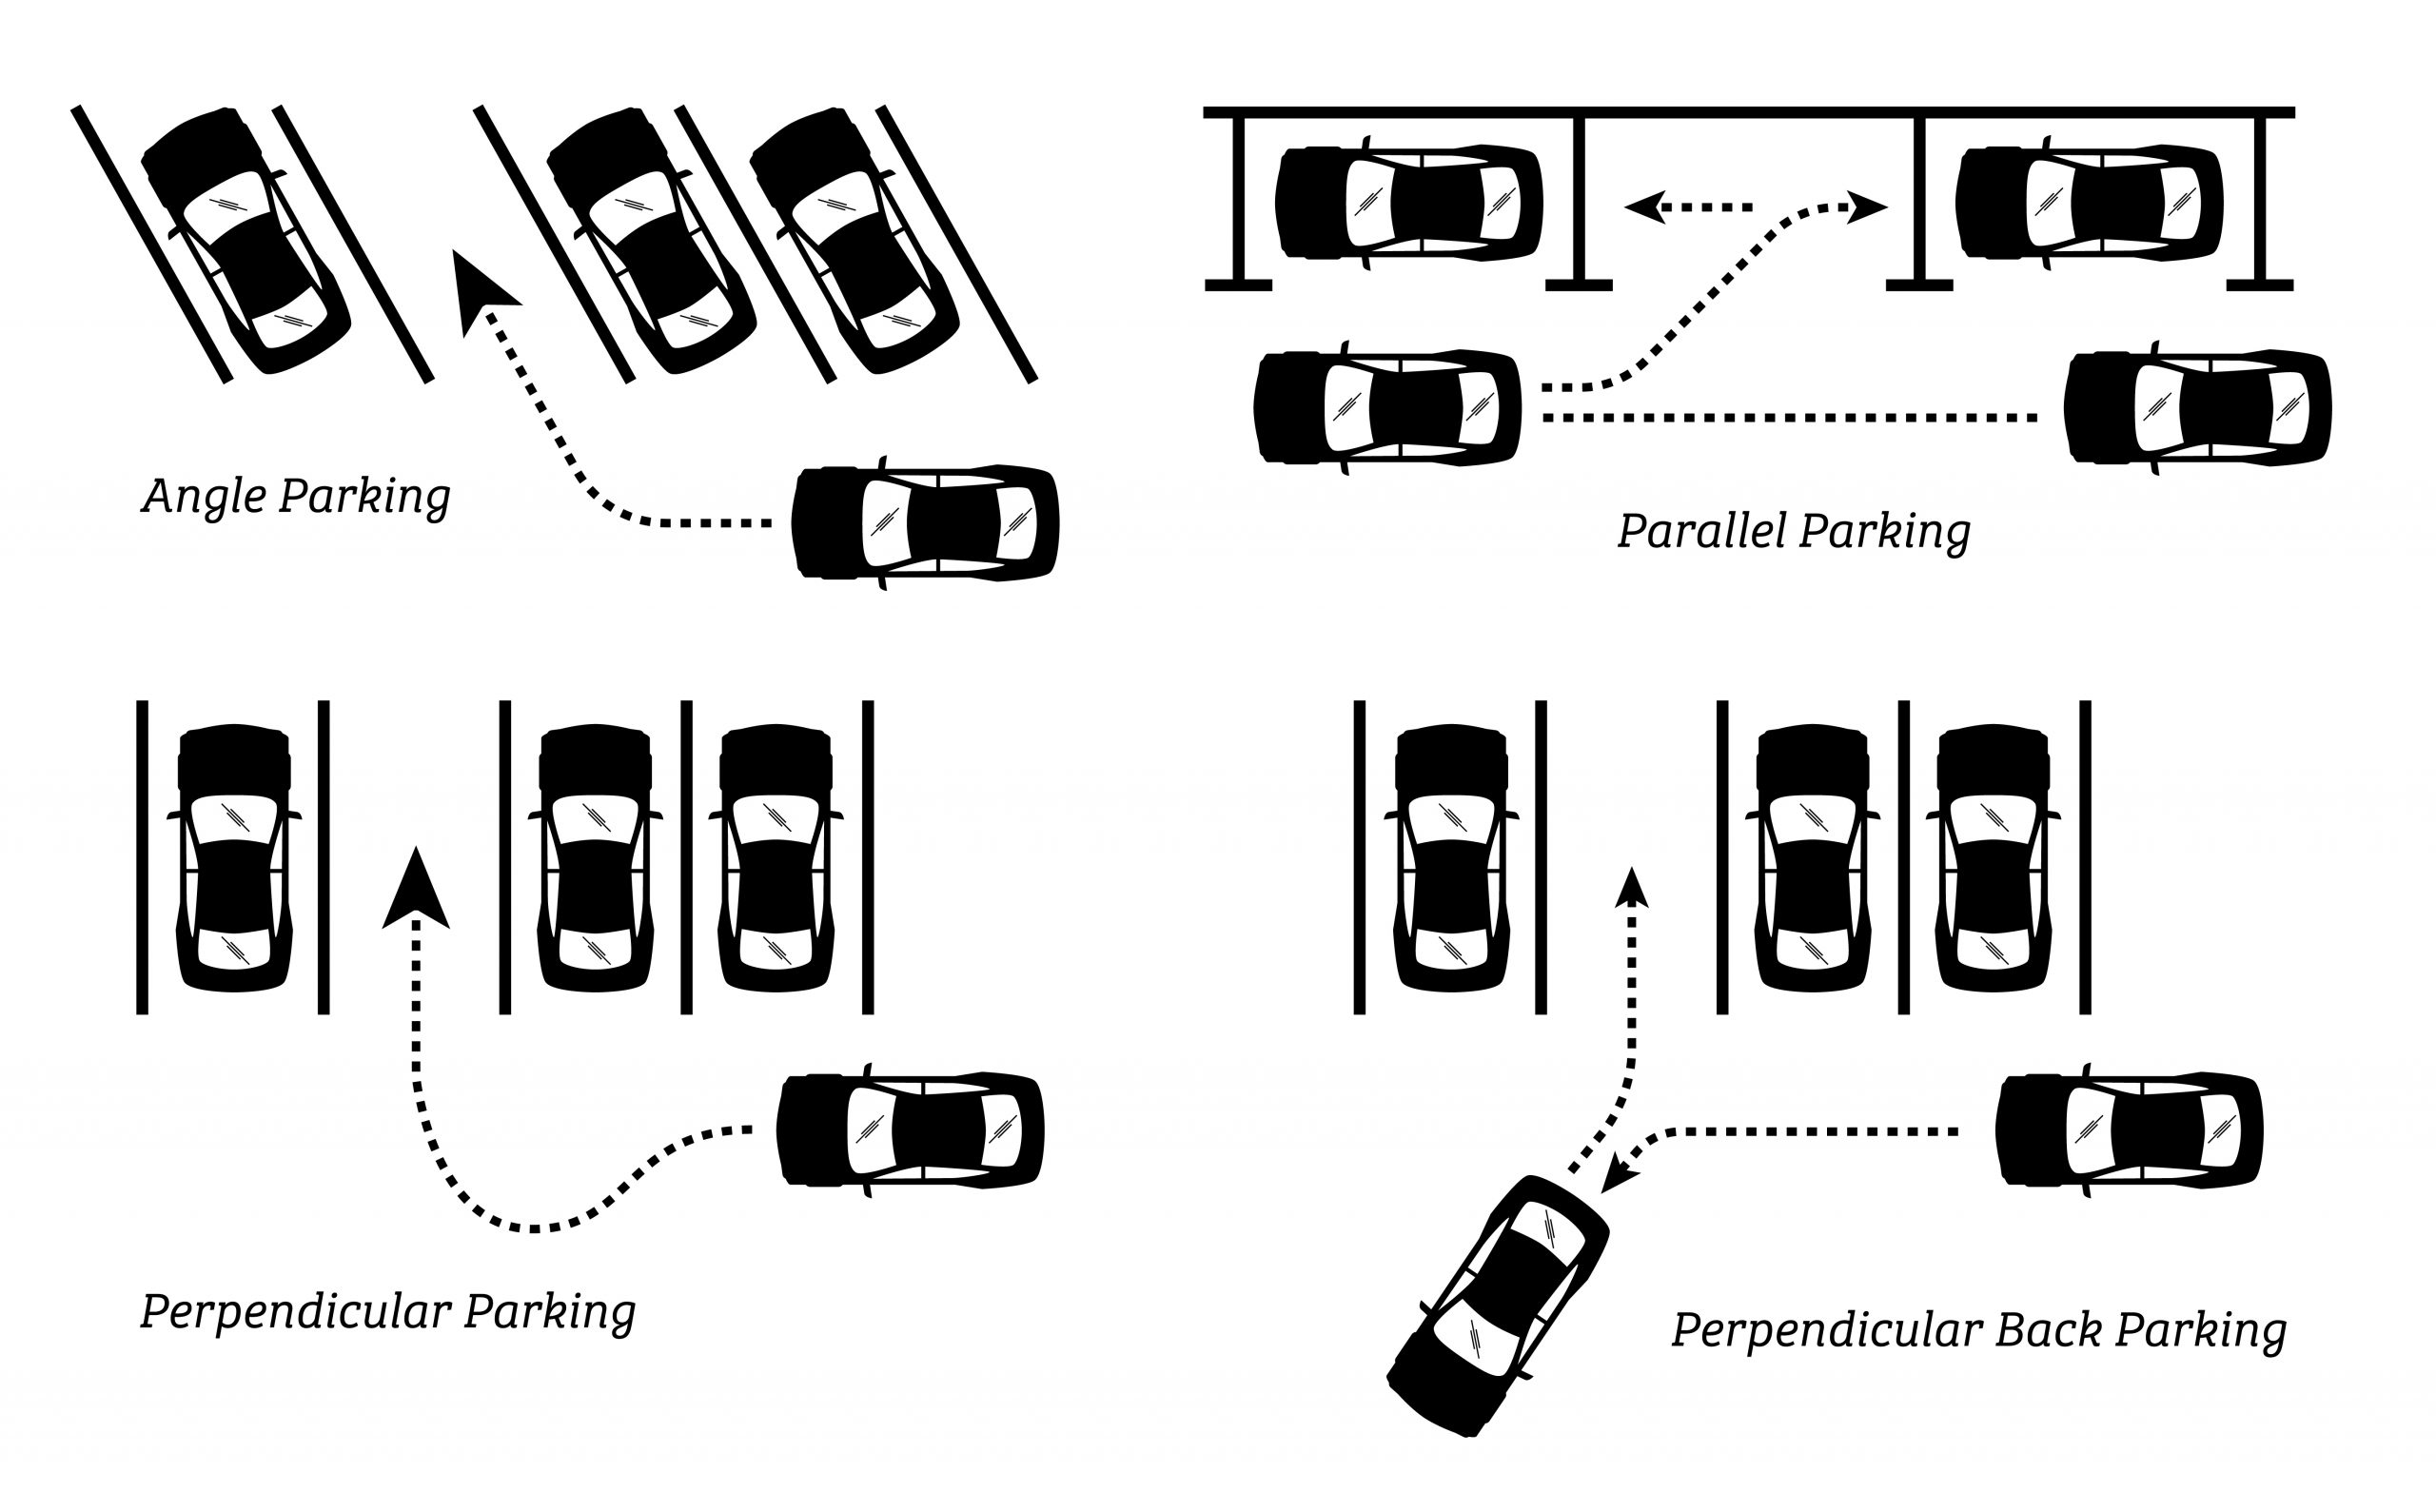
\includegraphics[width=4in]{images/Chap2/perpendicular-parking-a-lot-scaled.jpg}\\
    \caption{Parking Styles}
    \label{Parking Styles}
    \end{center}
\end{figure}

Analogically, after the truck arrives in the station, the drivers would drive and steer in the opposite direction of the 
pallet, until the forks are in a position to allow the truck to easily and correctfully drive to the pallet in fork direction.
The goal here is to develop a pallet-linking algorithm to automate the driving to the pallet pickup location for 
autonomous forklifts as given by figure \ref{pattern}. The truck would autonomously plan the path to its destination
based on the pattern and on the environment settings that it would navigate in. 
The pattern enhances the explainability in the forklifts behavior. Explainability allows for more order in the warehouse: 
it simplifies the coordination of safe simultaneous tasks around the truck. This is achieved through the design of an 
algorithm that aims to create a transparent navigation process, making it easier for humans to understand and trust 
the technology. Additionally, the approach is intended to ensure secure and reliable decision-making for autonomous trucks.



\begin{figure}
    [H]
    \begin{center}
    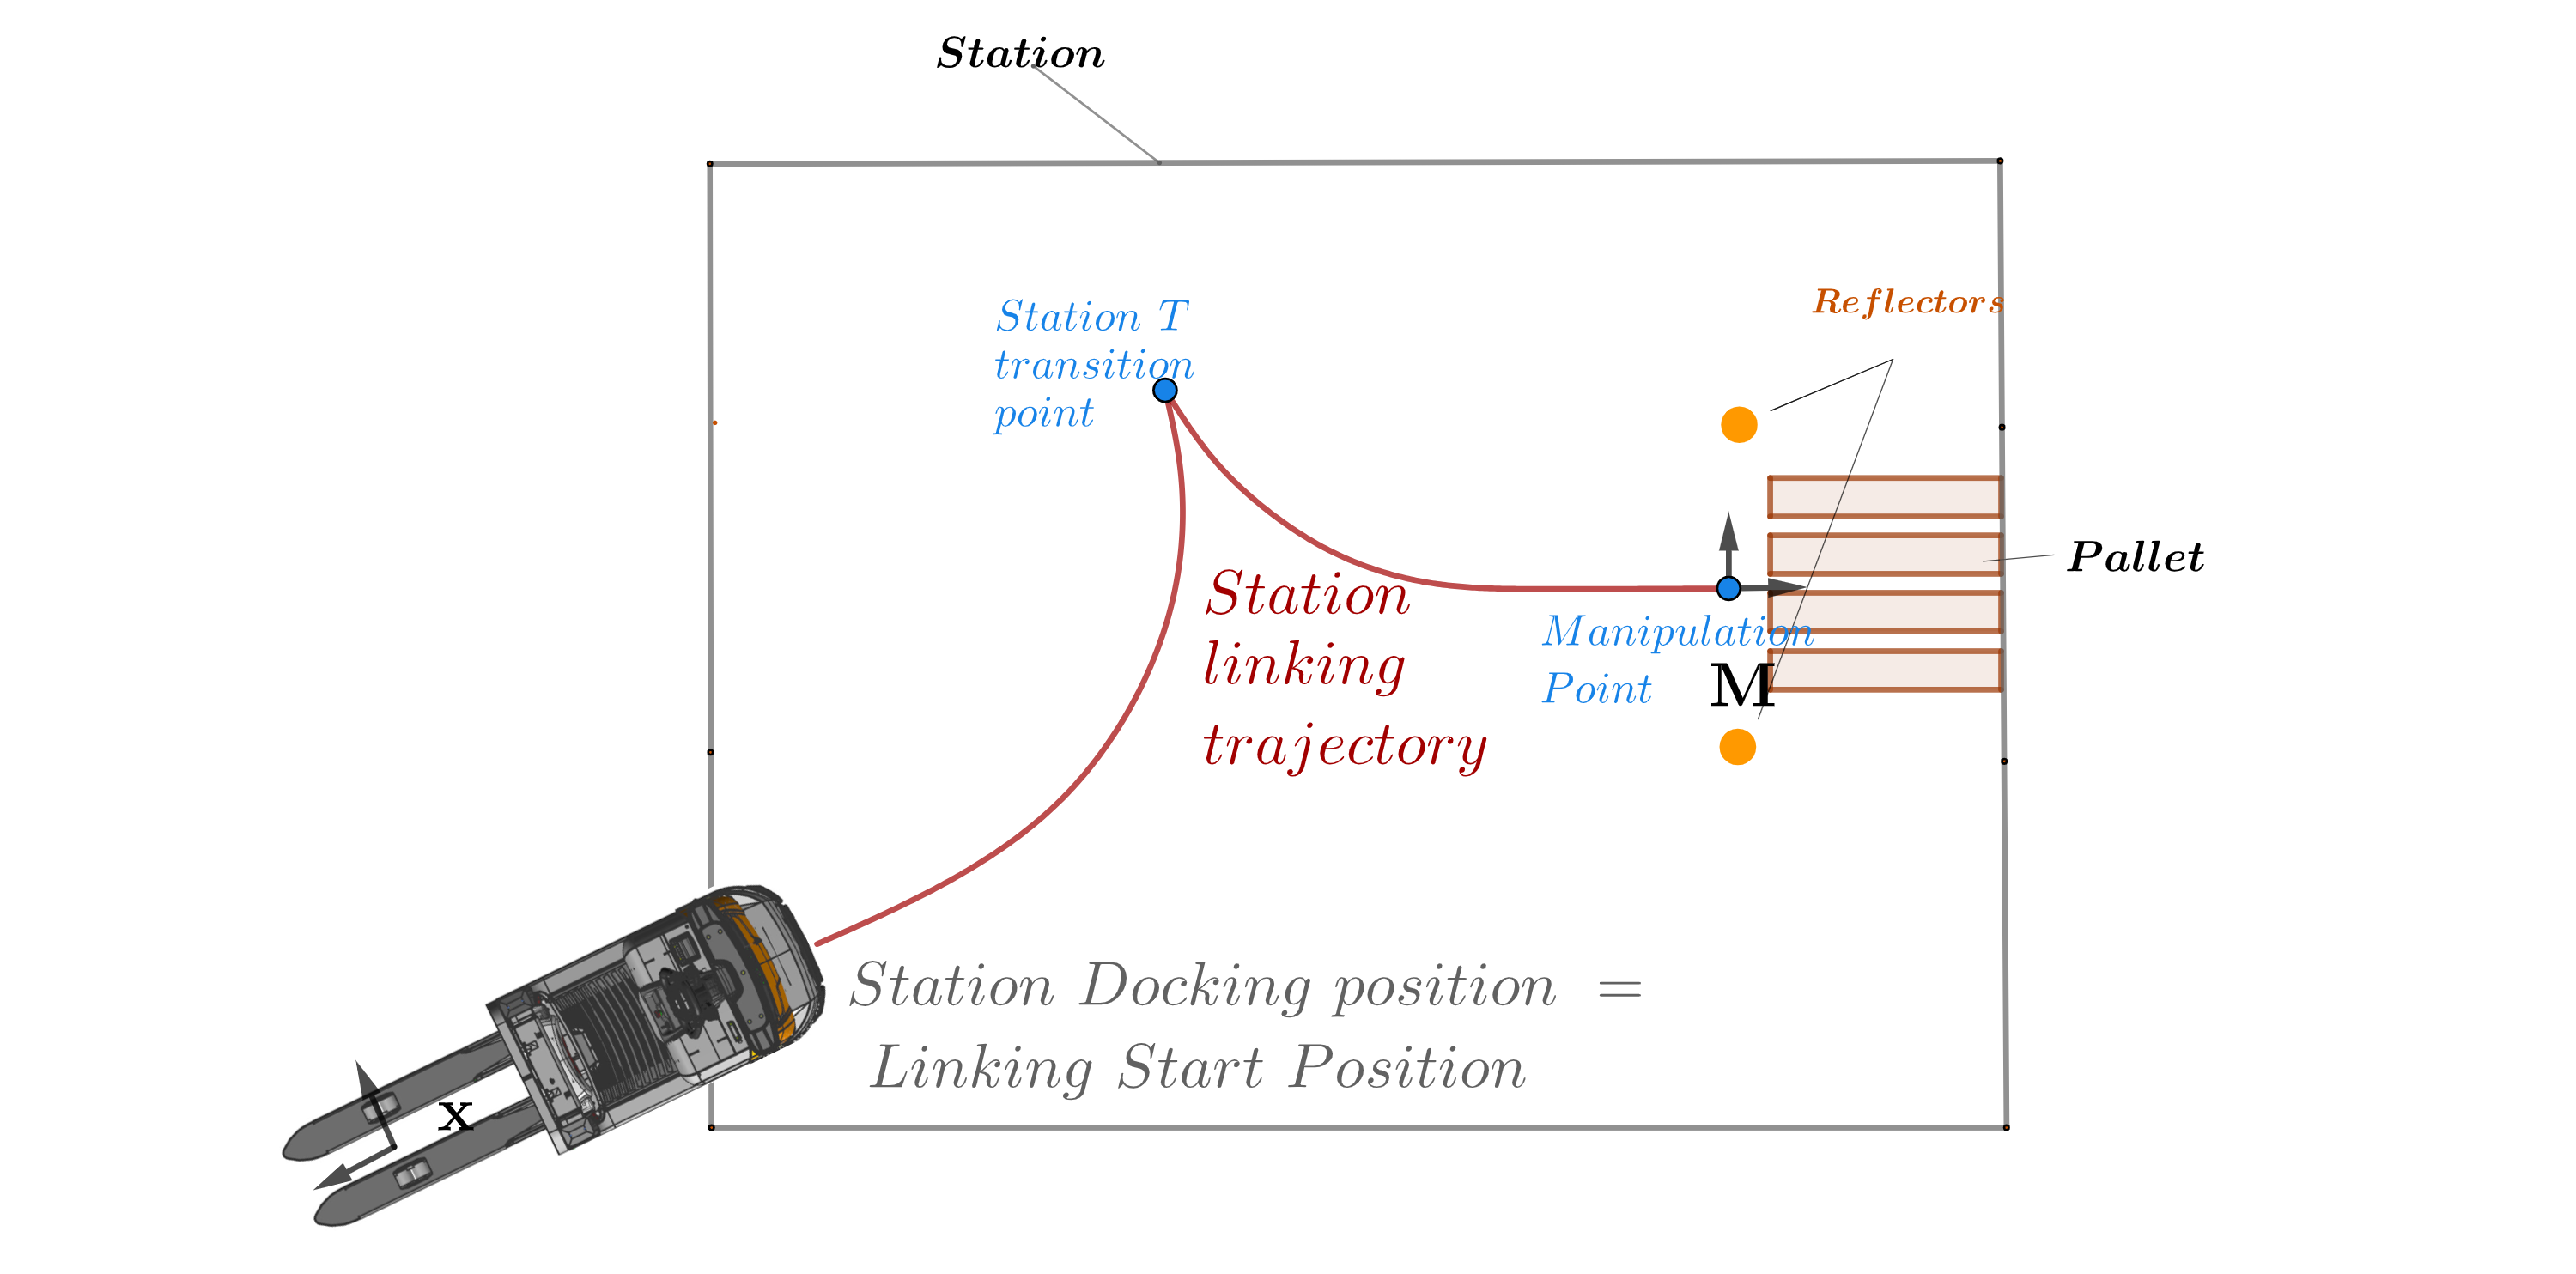
\includegraphics[width=\linewidth]{images/Chap2/station-without-subpolygones.png}\\
    \caption{Linking the robot to goal destination \cite{R28}}
    \label{pattern}
    \end{center}
\end{figure}
From now on, the following definitions of driving directions will be used as gven by figure \ref{driving directions}:
\begin{itemize}
    \item Main Driving Direction: Driving in fork direction.
    \item Opposite Driving Direction: Driving in vehicle chassis direction.
\end{itemize}

\begin{figure}
    [!ht]
    \begin{center}
    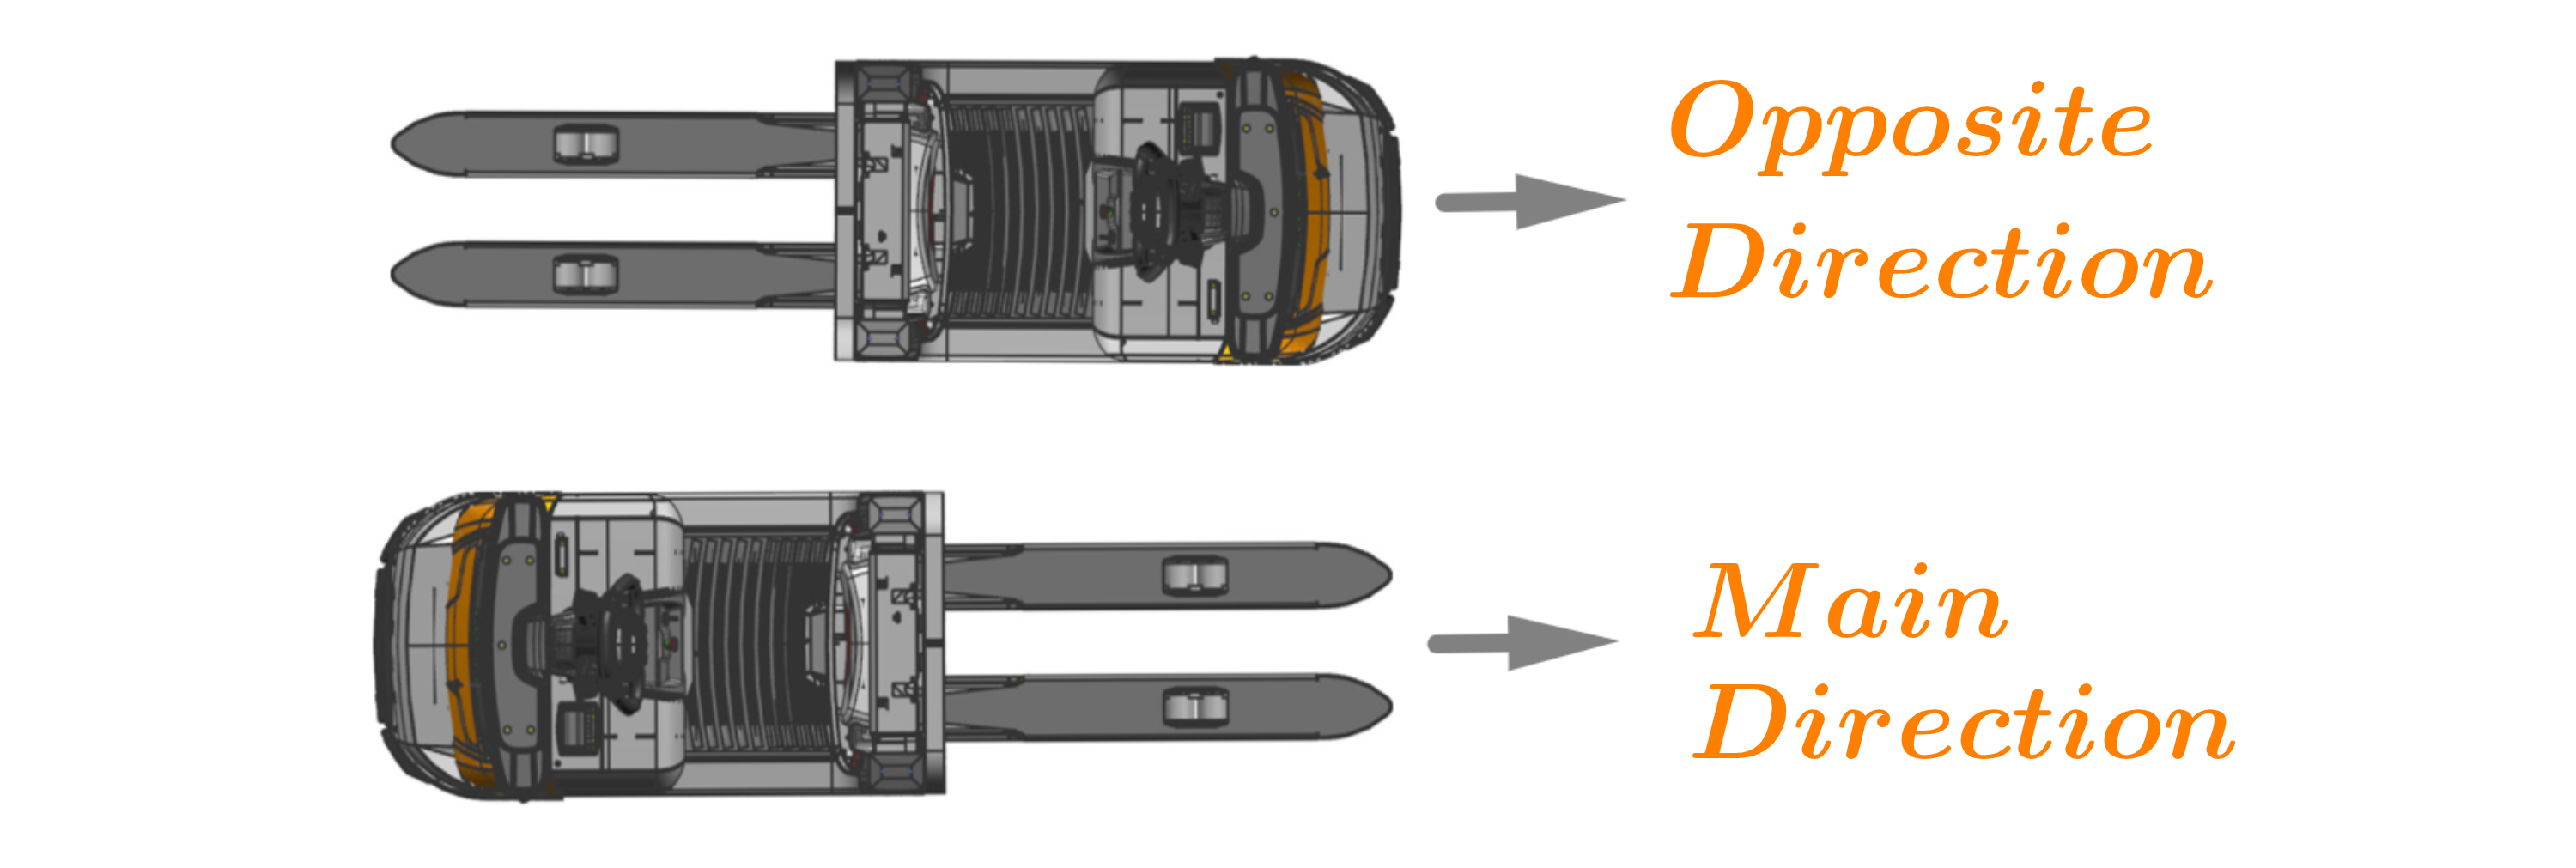
\includegraphics[width=4in]{images/Chap2/driving_directions.png}\\
    \caption{Truck Driving Directions}
    \label{driving directions}
    \end{center}
\end{figure} 
 
The following transition method is suggested: once the truck docks the station, it has the option to transition and change 
direction on the sides of the shelf placed inside the station. First, it drives to the transition position, then, to the 
pallet or the drop-off position as given by figure \Ref{subpolygons}. Having two possibilities for transition zones allows 
for more flexibility: 
in case one area is unreachable or presents obstacles, the second one can be used. They present free areas 
inside the stations where less obstacles and dynamics are expected and smooth maneuvering of the truck can be managed. 
In addition, the geometric solution is scalable to 
any station that is recognized and whose properties are available to the truck. This makes the overall solution and the 
autonomous forklifts simple to
commission in new warehouses.

\begin{figure}
    [!ht]
    \begin{center}
    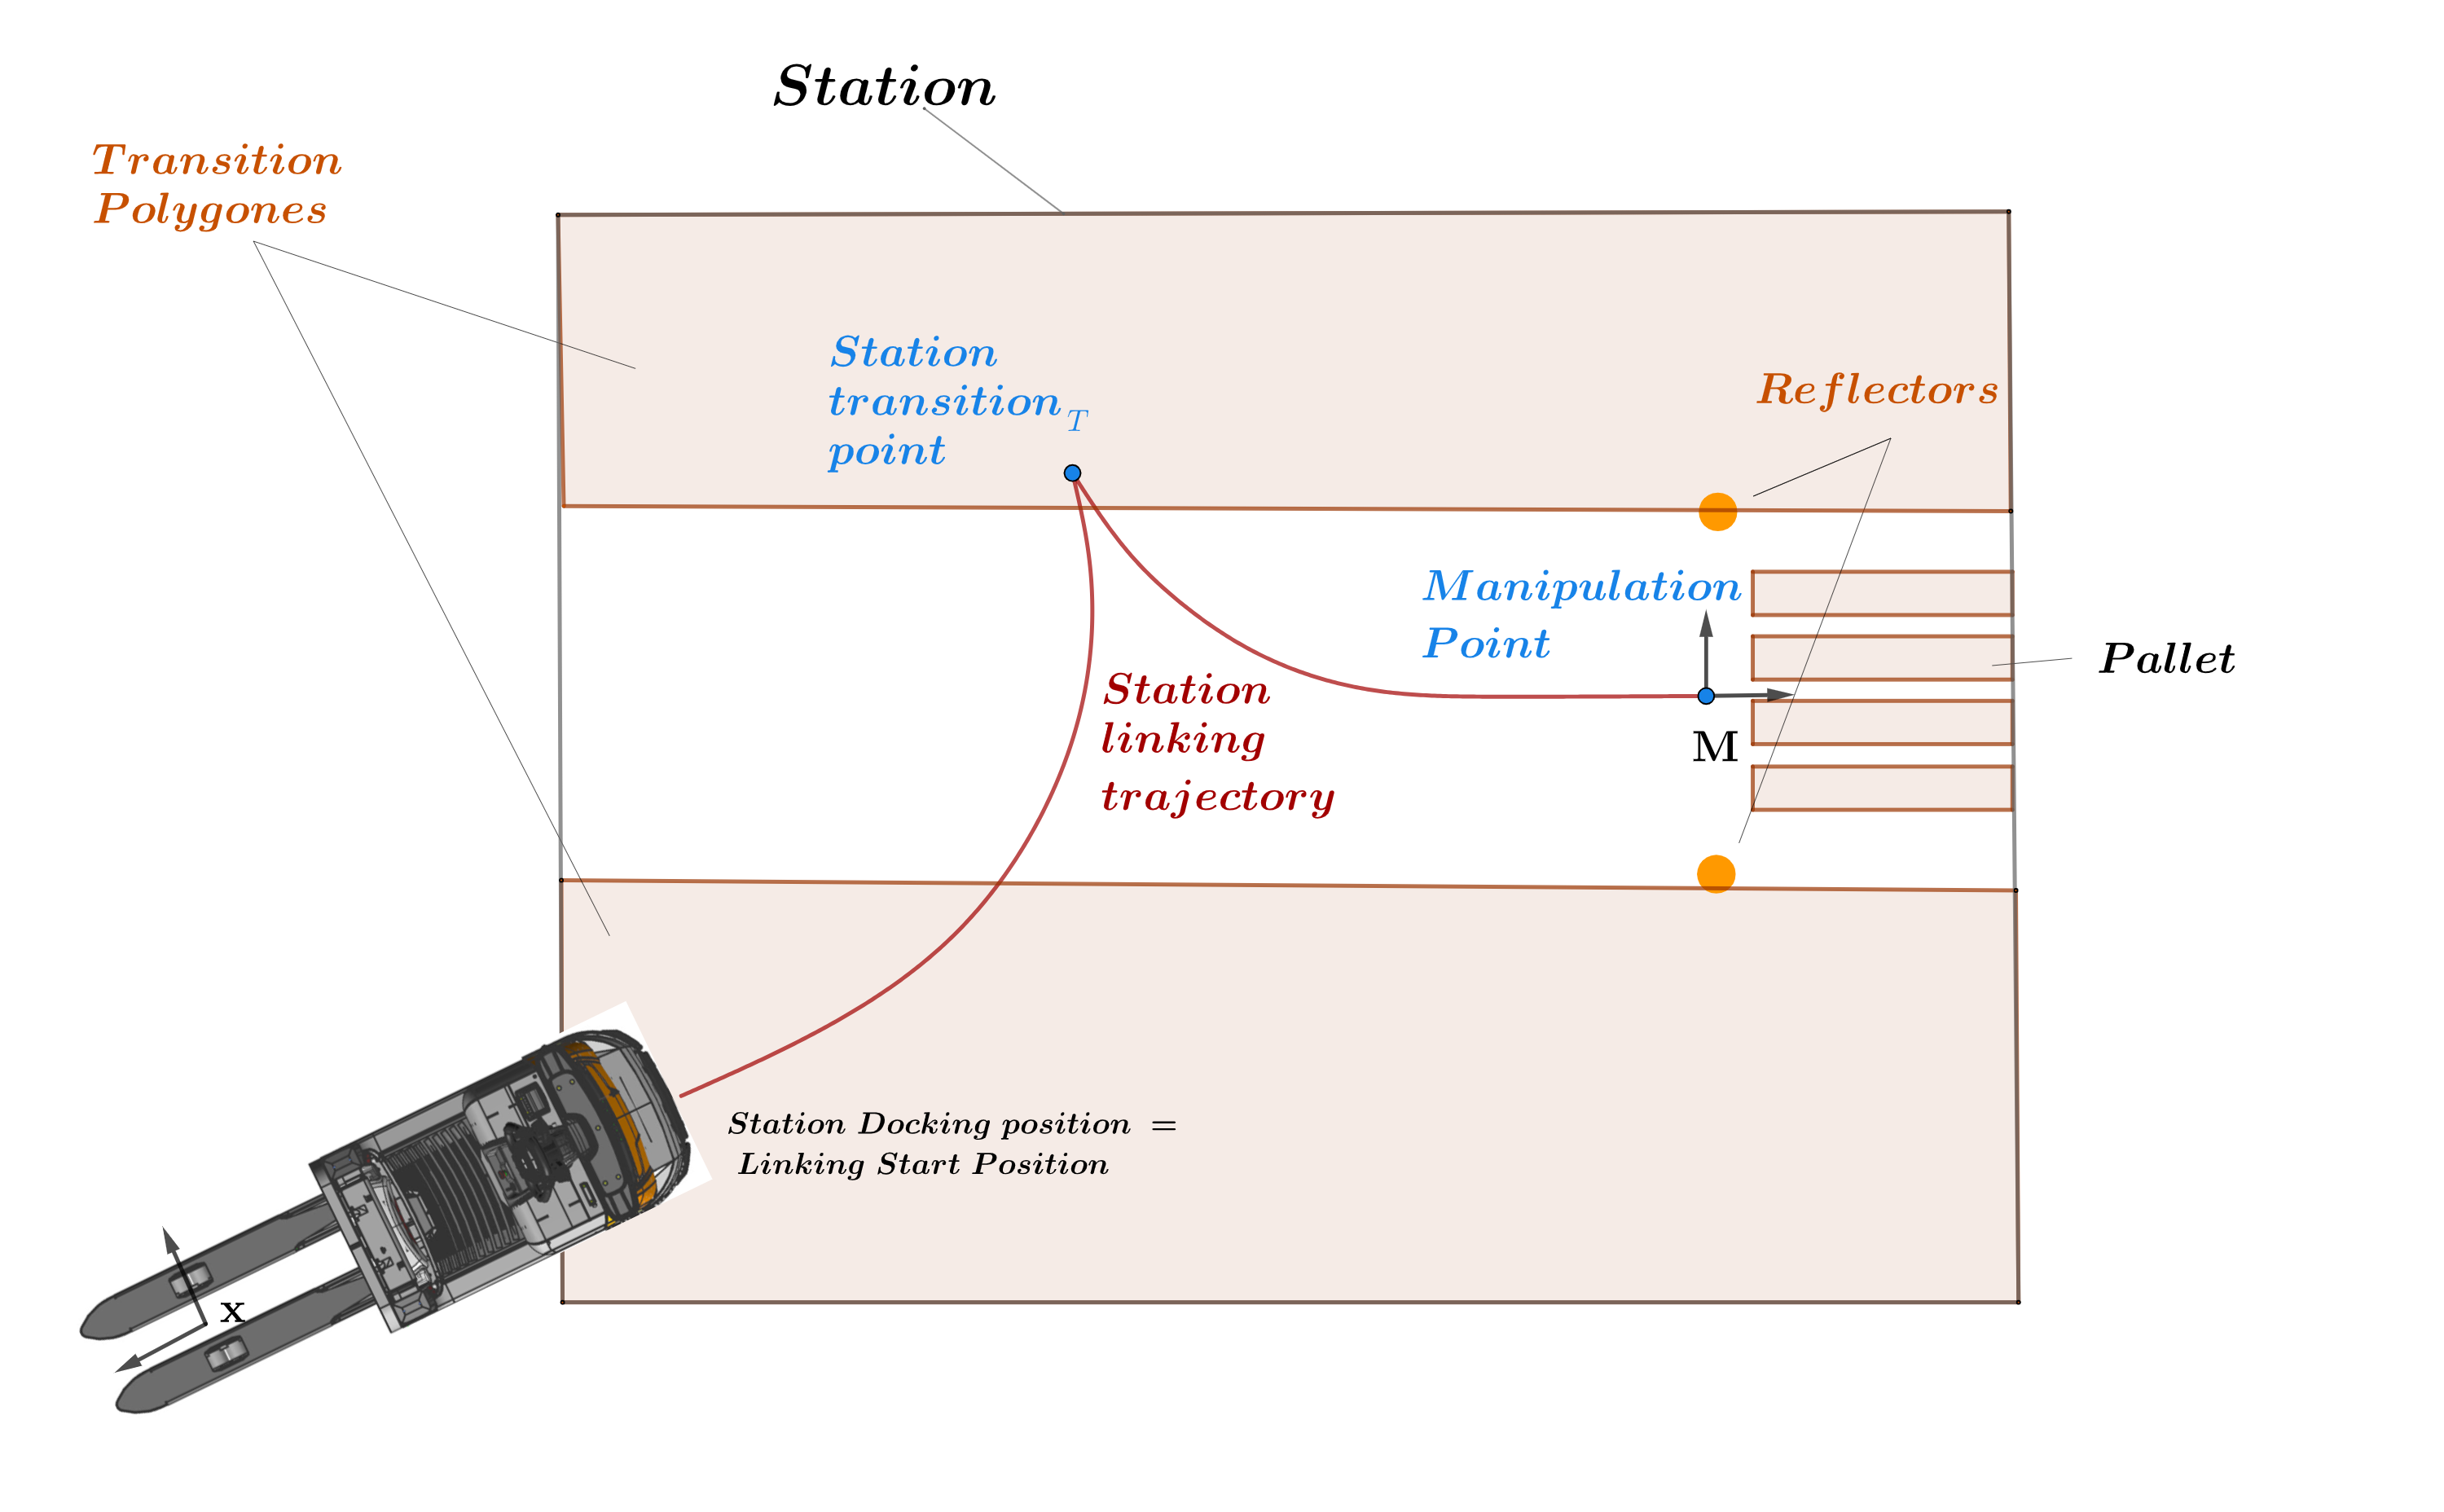
\includegraphics[width=\linewidth]{images/Chap2/station-without-subpolygones (2).png}\\
    \caption{Linking the robot to goal pallet \cite{R28}}
    \label{subpolygons}
    \end{center}
\end{figure}

Smooth and continuous paths are generated through spline interpolation of constructed waypoints. This technique ensures 
that the resulting paths are smooth, operationally seamless, and reduce abrupt changes in direction and speed. 
By interpolating between waypoints, the method enables the creation of curves that are optimized for driving efficiency 
and stability.

Finally, an optimizer generates an optimal path. 
generates multiple path candidates and rigorously evaluates each one based on key factors. 
The evaluation considers the path's length, smoothness, and potential collisions with surrounding objects to ensure the 
chosen path is both efficient and safe. After testing all options, the path that best meets these 
criteria—providing the shortest, smoothest, and safest route with minimal collision risk—is selected as the best solution. 

This approach ensures the final path is not only theoretically ideal but also practical and reliable for real-world use. 
The process is designed to be flexible and effective, even in obstacle environments. The designed methodology 
is summarized in the following flowchart \ref{design}:

\begin{figure}[!ht]
    \begin{center}
        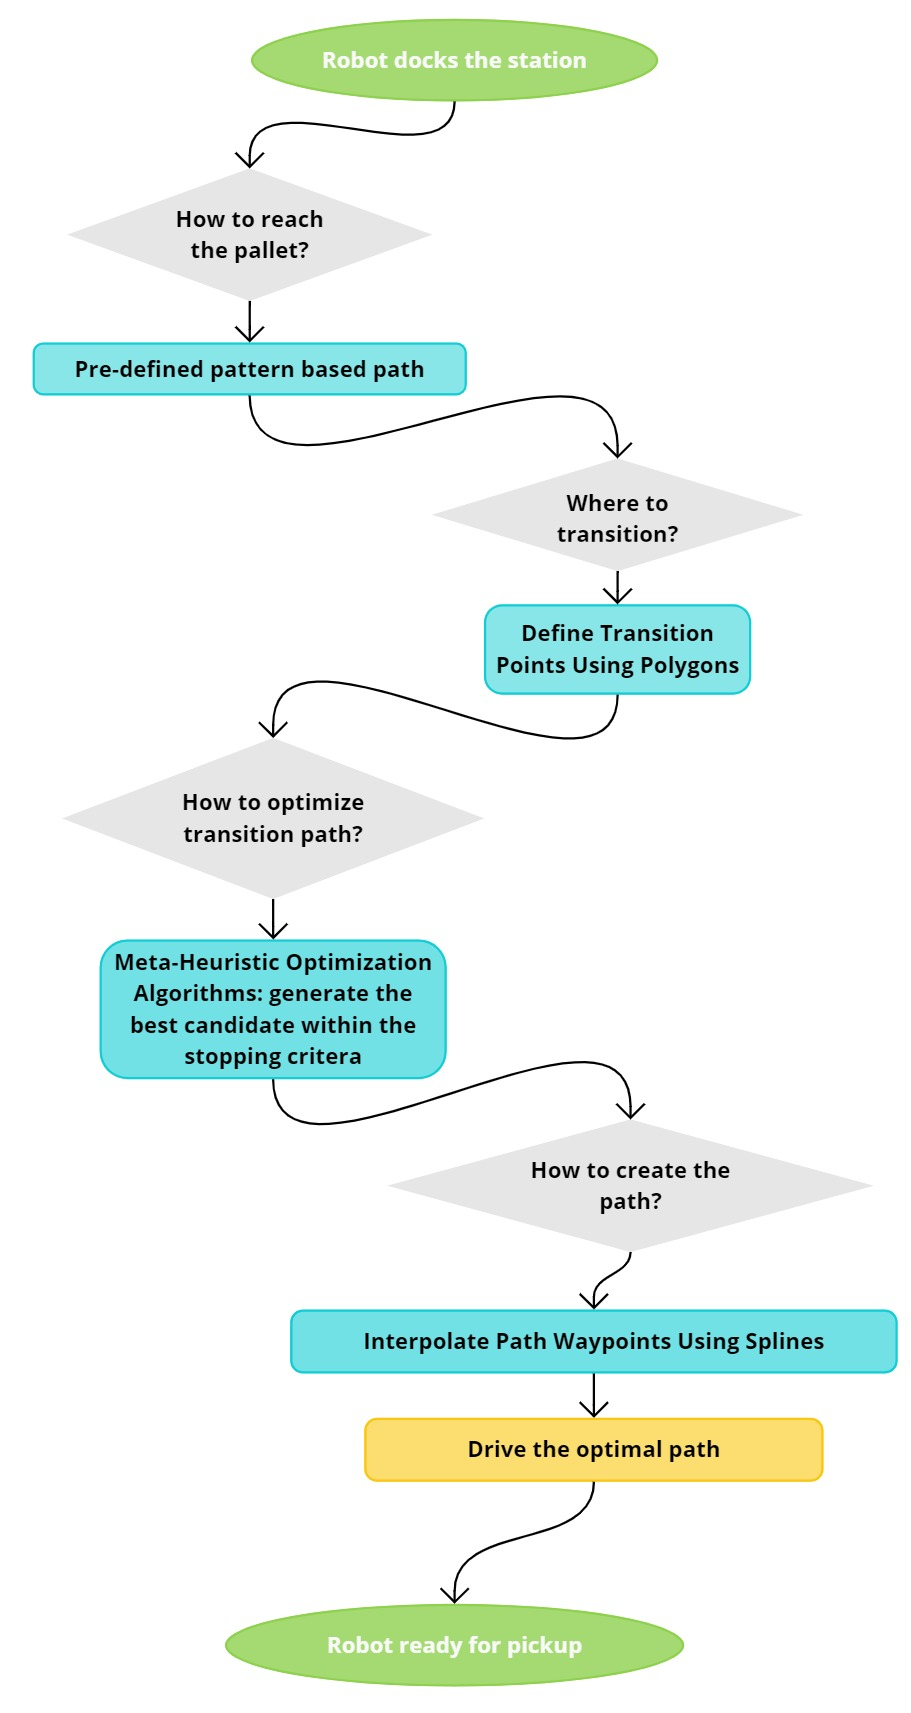
\includegraphics[width=4in]{images/Chap2/Approch_design.jpg}\\
        \caption{Path planning approach to pallet docking}
        \label{design}
        \end{center}
\end{figure}

\section{Development phases and Implementation}

This section details the rollout of the module development, providing a comprehensive overview of the process. 
It is structured to include both the development steps and the corresponding simulation results at each phase.
Every phase started with a deep investigation of the existing relevant solutions detailed in Chapter 2.

\subsection{Geometric Partitioning of the Station}
This section explains the development of the geometric Partitioning of the station into 2 polygons used later for 
transitioning inside the station. \textbf{The input of this step is the station information and the output are the polygons}.
\subsubsection{Utility}
As explained previously in Section 3.2, in order to carry out the transitioning of the vehicle inside 
the station to change the driving direction from the opposite to the main direction, Transition subpolygons are needed. 
The subpolygons are created according to the station shape and dimensions and the position of the shelf inside of it. 
As given by figure \ref{warehouse}, the stations can be found at certain positions of the warehouse.

\subsubsection{Implementation}
The vehicle initially plans its missions: it constructs a plan of the stations that will be visited and the operations
to do on each station. While the path driven from one station to the other is pre-defined by the global planner, 
the path linking the vehicle to the pallet is to be planned in real-time. 
Once the vehicle arrives at the docking position in the stations, it starts the path planning process. 
The station-related information are stored in a file accessible to the vehicle. These information include, but are 
not limited to, it position and dimensions and the coordinates of the shelf that it contains.
For each station represented like figure \ref{Station} the module creates the subpolygons on each side of the shelf, 
limited by the station and shelf shapes. 

The process that creates the subpolygons is detailed in the following Algorithm \ref{alg:createSubpolygons}.
The algorithm begins with an initialization step, then the corners of the station and shelf areas are retrieved and 
transformation matrices are prepared to convert coordinates between global and shelf-specific coordinate systems. 
The need to transform the used coordinates to the shelf frame is derived from the scalability needs.
As seen on figure \Ref{warehouse}, stations can be placed in different positions and have different orientations.
If global coordinates are used, it becomes computationally challenging to develop an exhaustive algorithm that fits all the 
possibilities of station orientation and shelf positioning. On the other hand, using the shelf coordinate frame shifts 
the point of view to the inside of the station only. It enables the shelf to orchestrate the geometric partitioning 
of the station based on its position in the station.
The algorithm then iteratively transforms the station and shelf corners from global coordinates to shelf coordinates, 
storing the transformed corners in dedicated lists. After the transformation, two subpolygons are created: one 
representing the negative Y subpolygon (NegYsub\_polygon) and the other representing the positive Y subpolygon
(PosYsub\_polygon). For special cases like station3, where one of the subpolygons can be very narrow (lower than a 
certain threshhold), the algorithm omits it and generates only one subpolygon. 
The algorithm concludes by returning the created subpolygon(s), effectively segmenting the 
input areas into distinct, usable geometric entities.


\begin{figure}[H]
    \begin{center}
        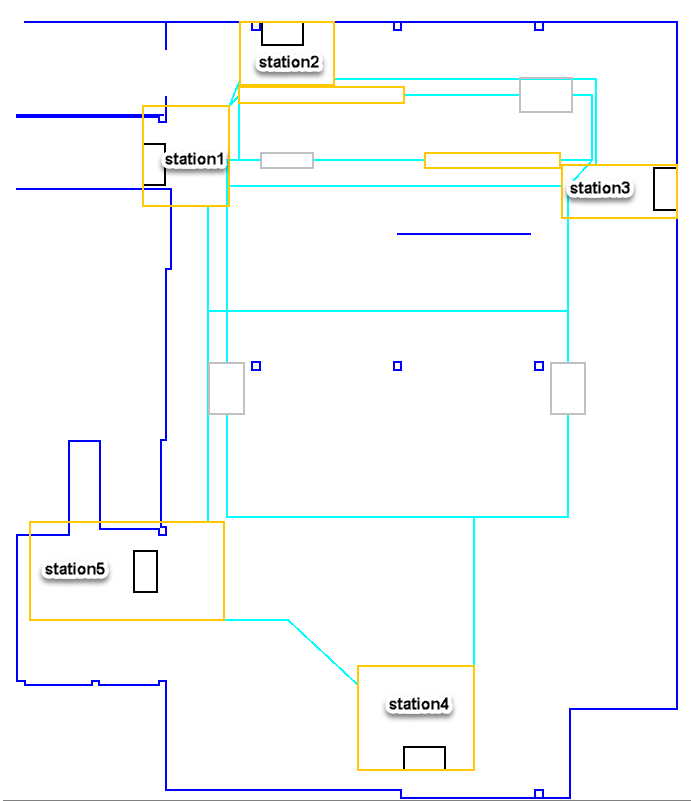
\includegraphics[width=4in]{images/Chap2/warehouse.png}\\
        \caption{Simulation of the stations in a warehouse}
        \label{warehouse}
        \end{center}    
\end{figure}



\begin{figure}[H]
    \begin{center}
        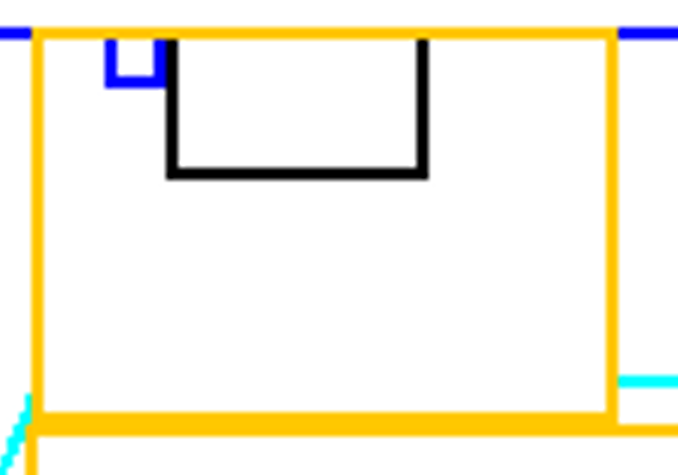
\includegraphics[width=3in]{images/Chap2/station.png}\\
        \caption{Station Simulation}
        \label{Station}
        \end{center}    
\end{figure}


\noindent

\begin{algorithm}
\caption{Creation of Subpolygons}\label{alg:createSubpolygons}
\KwData{station\_area, shelf\_area}
\KwResult{created two subpolygons}
\BlankLine
\textbf{Initialization}; \\
station\_corners, shelf\_corners $\gets$ GetCorners(station\_area, shelf\_area)\;
tm\_station\_corners, tm\_shelf\_corners $\gets$ empty lists\;
tm\_shelf2global $\gets$ GetTransMatrix(shelf\_area)\;
tm\_global2shelf $\gets$ InvertMatrix(tm\_shelf2global)\;
\ForEach{corner $\in$ station\_corners}{
    corner\_shelf $\gets$ TransformCorner(tm\_global2shelf, corner)\;
    tm\_station\_corners.append(corner\_shelf)\;
}
station\_corners\_shelf.append(tm\_station\_corners[0])\;
\ForEach{corner $\in$ shelf\_corners}{
    corner\_shelf $\gets$ TransformCorner(tm\_global2shelf, corner)\;
    tm\_shelf\_corners.append(corner\_shelf)\;
}
NegYsub\_subpolygon $\gets$ CreateNegYsubpolygon(tm\_station\_corners, tm\_shelf\_corners, tm\_shelf2global)\;
PosYsub\_subpolygon $\gets$ CreatePosYsubpolygon(tm\_station\_corners, tm\_shelf\_corners, tm\_shelf2global)\;
\Return{created two subpolygons}\;
\end{algorithm}
\noindent



\subsubsection{Results}

In figure \ref{Station polygon} stands the simulated result processed using real station data: In purple and orange are 
the polygons, and in green the outer polygon represenst the station.

\begin{figure}[H]
    \begin{center}
        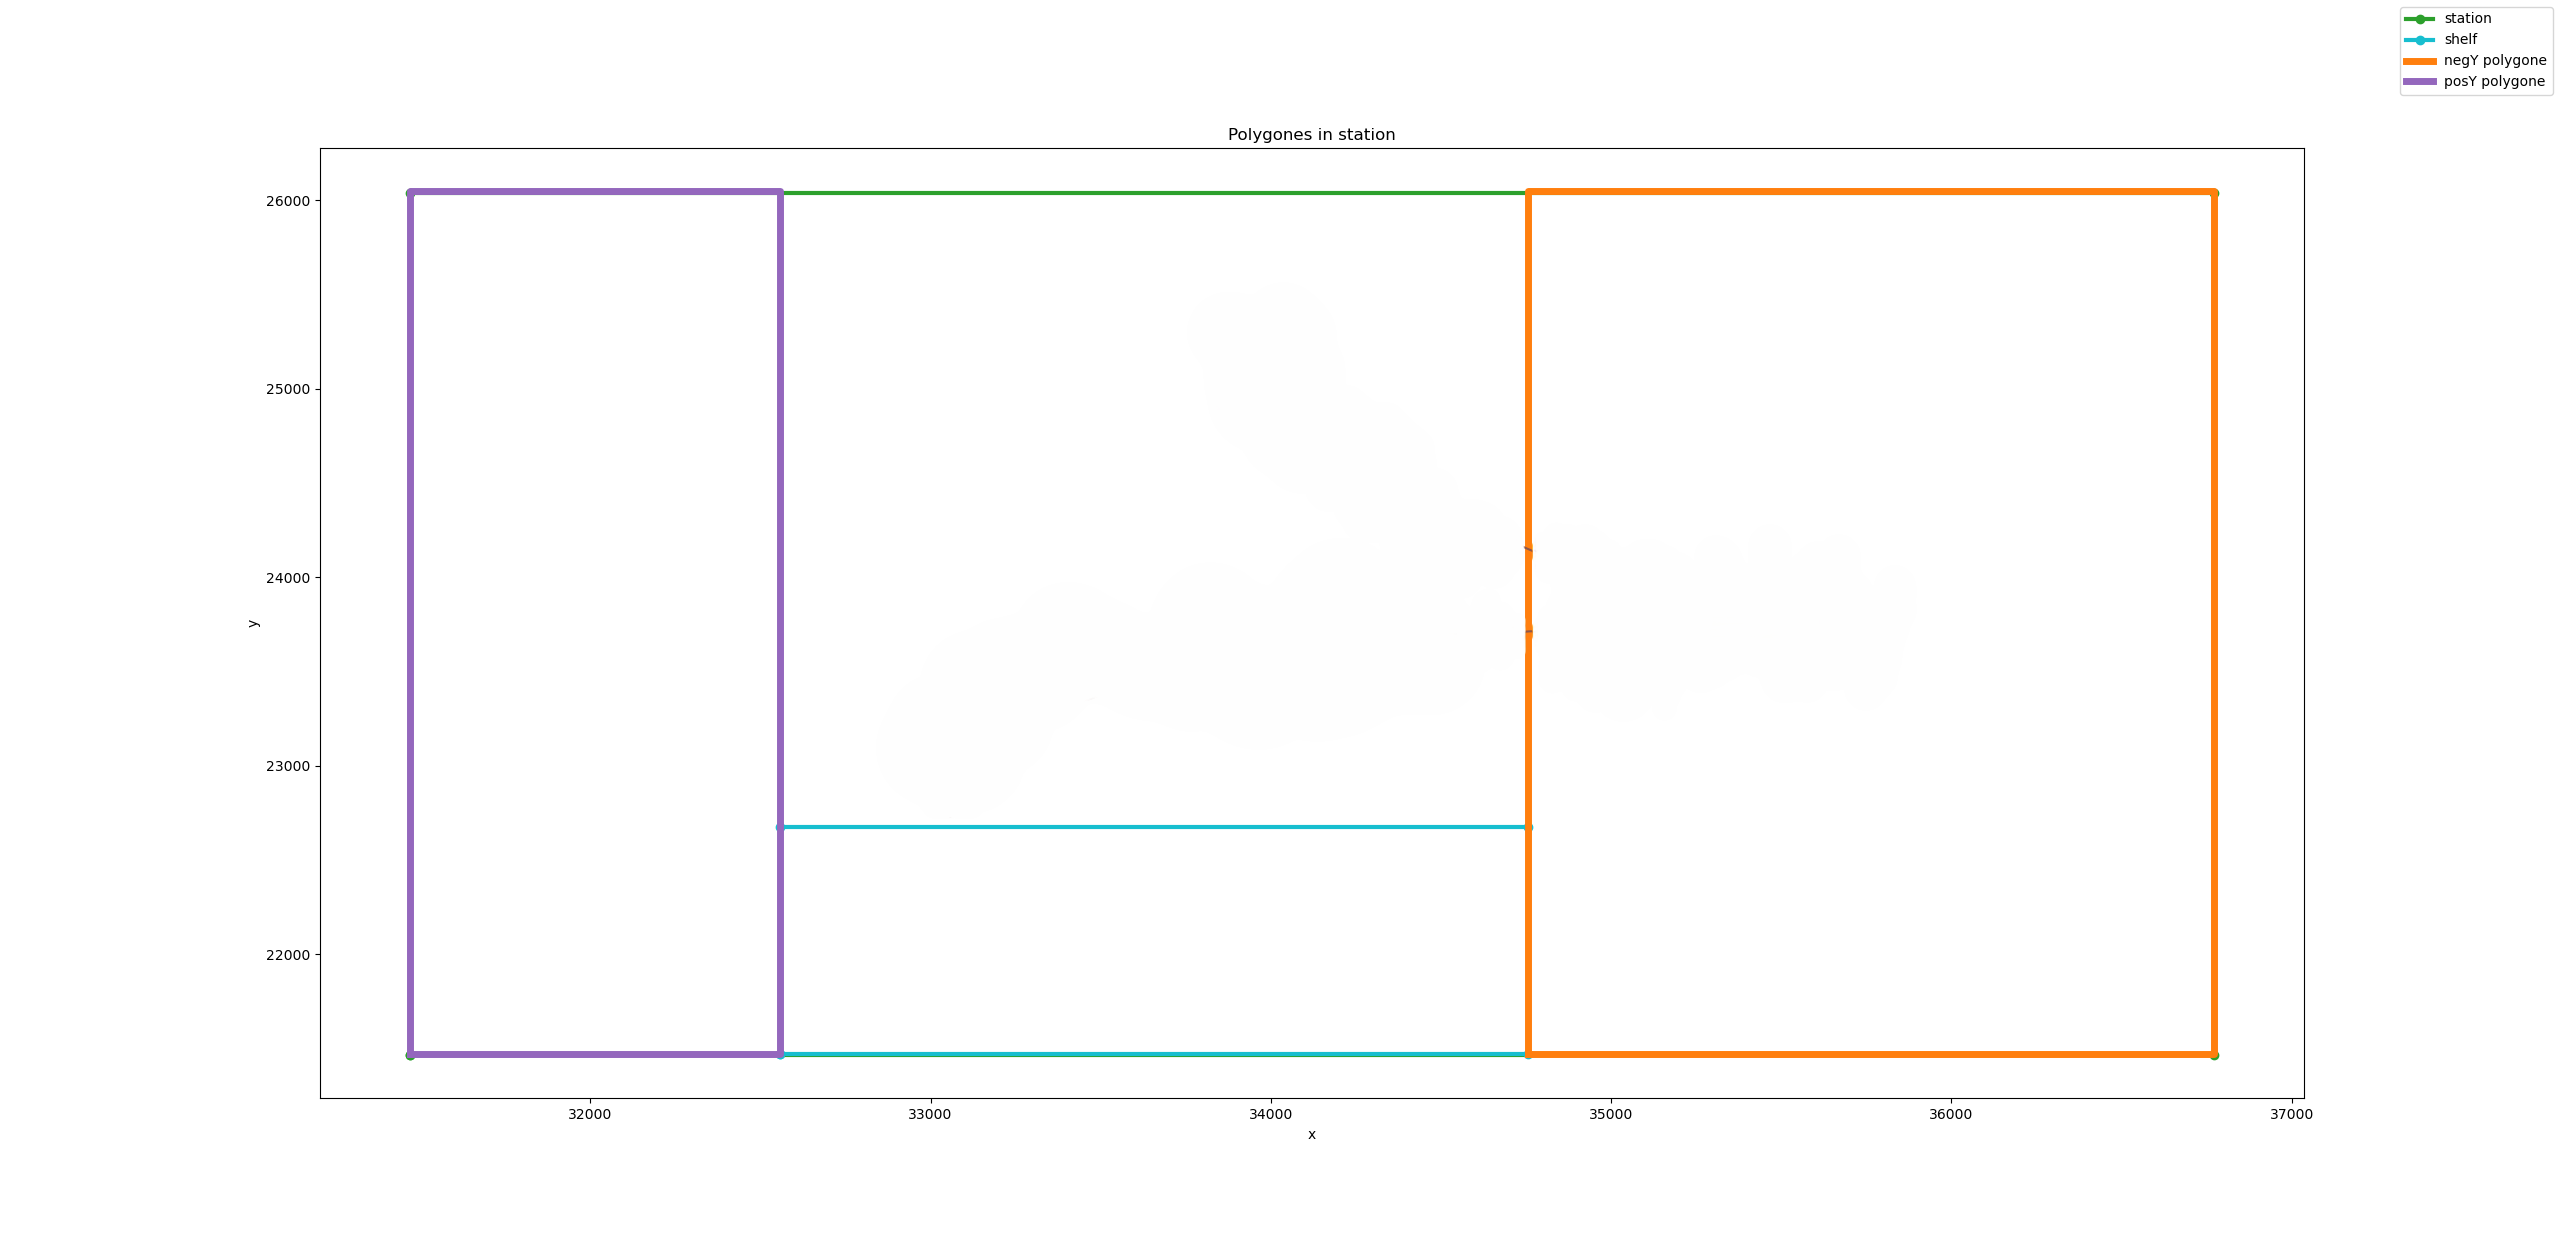
\includegraphics[width=5in]{images/Chap2/Polygons_created.png}\\
        \caption{Station with created Polygons}
        \label{Station polygon}
        \end{center}    
\end{figure}

In figure \Ref{other station}, stands the result of the module Create subpolygon in a different station:
\begin{figure}[H]
    \begin{center}
        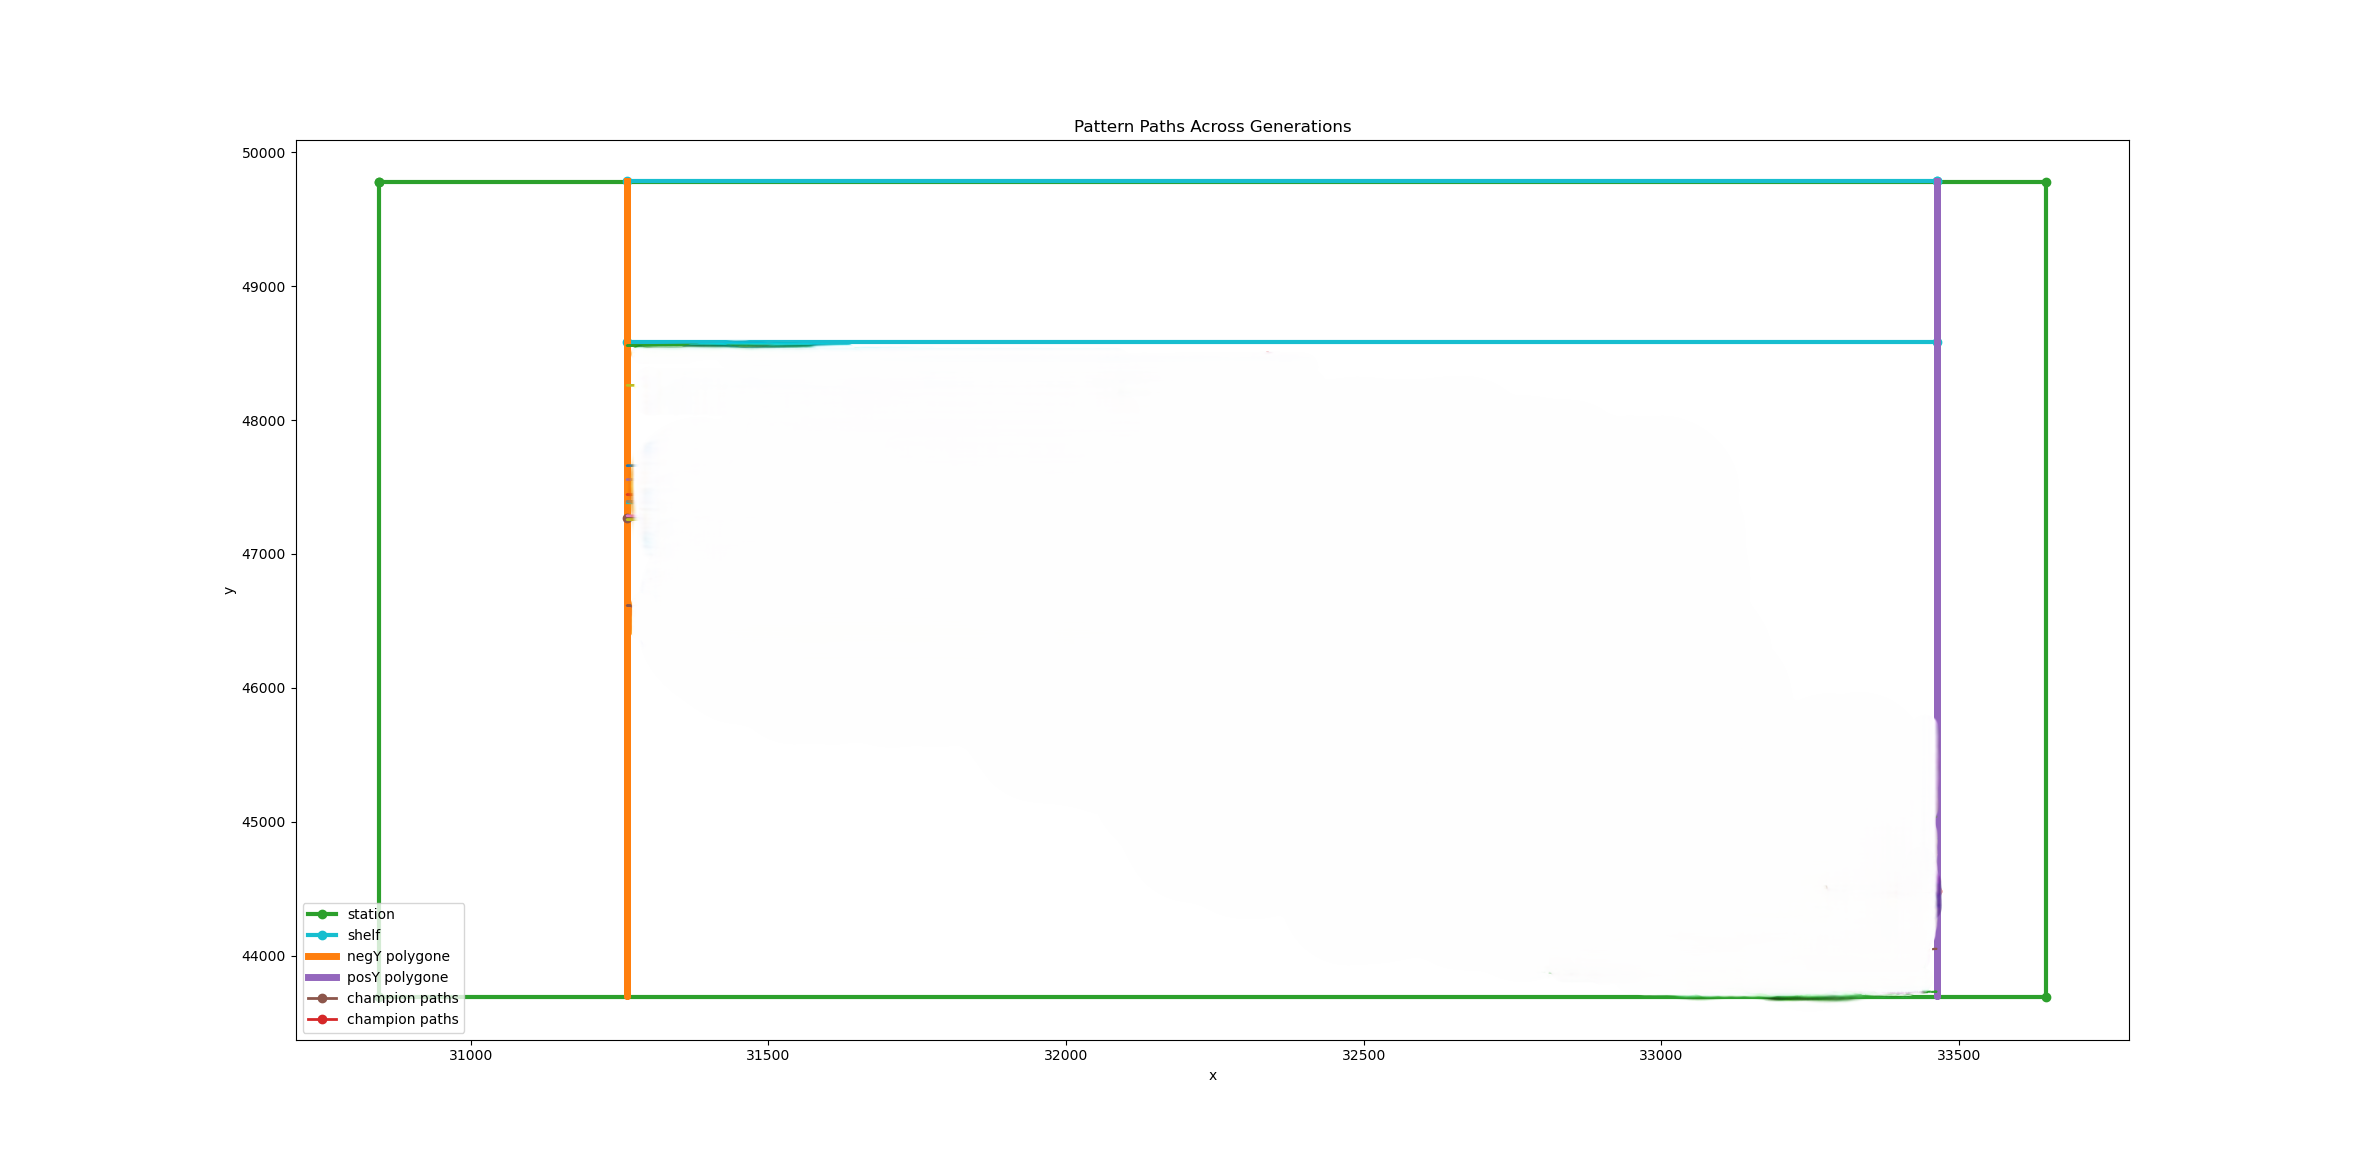
\includegraphics[width=5in]{images/Chap2/Other_station.png}\\
        \caption{Station with created Polygons}
        \label{other station}
        \end{center}    
\end{figure}
In figure \ref{} stands a plotted message that shows the creation of the polygons with their coordinates.

\subsection{Path creation}
This section details the methodology for path creation using splines. \textbf{The input of this section are the polygons besides
the robot's position and the destination. The output is a spline-based path linking the robot to the destination with a 
driving direction change}.

\subsubsection{Utility}

Spline-based paths provide several key benefits for robotic navigation. They ensure smooth and continuous movement by 
creating curved paths that connect waypoints seamlessly. Unlike abrupt turns and sharply angled paths, this smoothness 
reduces wear on the robot and makes its movements more energy-efficient. Additionally, spline-based paths make it 
easier to control the robot in real-time, allowing for quick adjustments if the environment changes and preventing 
oscillations as a response to control corrections. Using mathematical 
equations to define these paths also makes it simple to calculate important 
properties like path length and curvature, helping the robot navigate efficiently and safely. 

\subsubsection{Implementation}

Path creation comes after the creation of the subpolygons. After a transitioning point is chosen (see section %TODO
Path optimization), the waypoints are created. The waypoints depicted on the simulation figure \ref{Orientation} are created relating to the 
Robot, the destination and the transition positions. In a simple scenario where no obstacles are present, orientation points 
are strategically added in front of the three key positions of the robot. These orientation points serve as reference markers 
that guide the robot's movement, particularly during the initial phase of acceleration or deceleration. When the robot starts 
to move, it follows a precise trajectory, either in a straightforward or straight-backward direction, depending on the 
intended driving direction. This straight-line motion ensures that the robot maintains stability and accuracy as it 
transitions from a stationary position to motion or vice versa, minimizing any unnecessary deviations or turns that could 
disrupt its path. The alignment with the orientation points helps the robot to consistently maintain a straight trajectory, 
which is crucial for precise navigation and control.

Then, the orientaion points are interpolated to create the spline-based path. Given the need to create the driving direction 
change as a straight section of the path, two different splines will be interpolated using 4 waypoints each:
\begin{itemize}
    \item The first spline interpolates the starting points then the transition points.
    \item The second spline interpolates the transition points then the destination points.
\end{itemize}

By doing so, two connected splines are obtained. Then they are merged together in the same path data structure to 
form one path. The first spline is driven in opposite direction driving, the second in main direction driving. 
The transition section at the polygon enables the robot to have a positioning that facilitates changing the driving direction
as given by figure \Ref{transition}.

%TODO: remove white space from the next figures
\begin{figure}[H]
    \begin{center}
        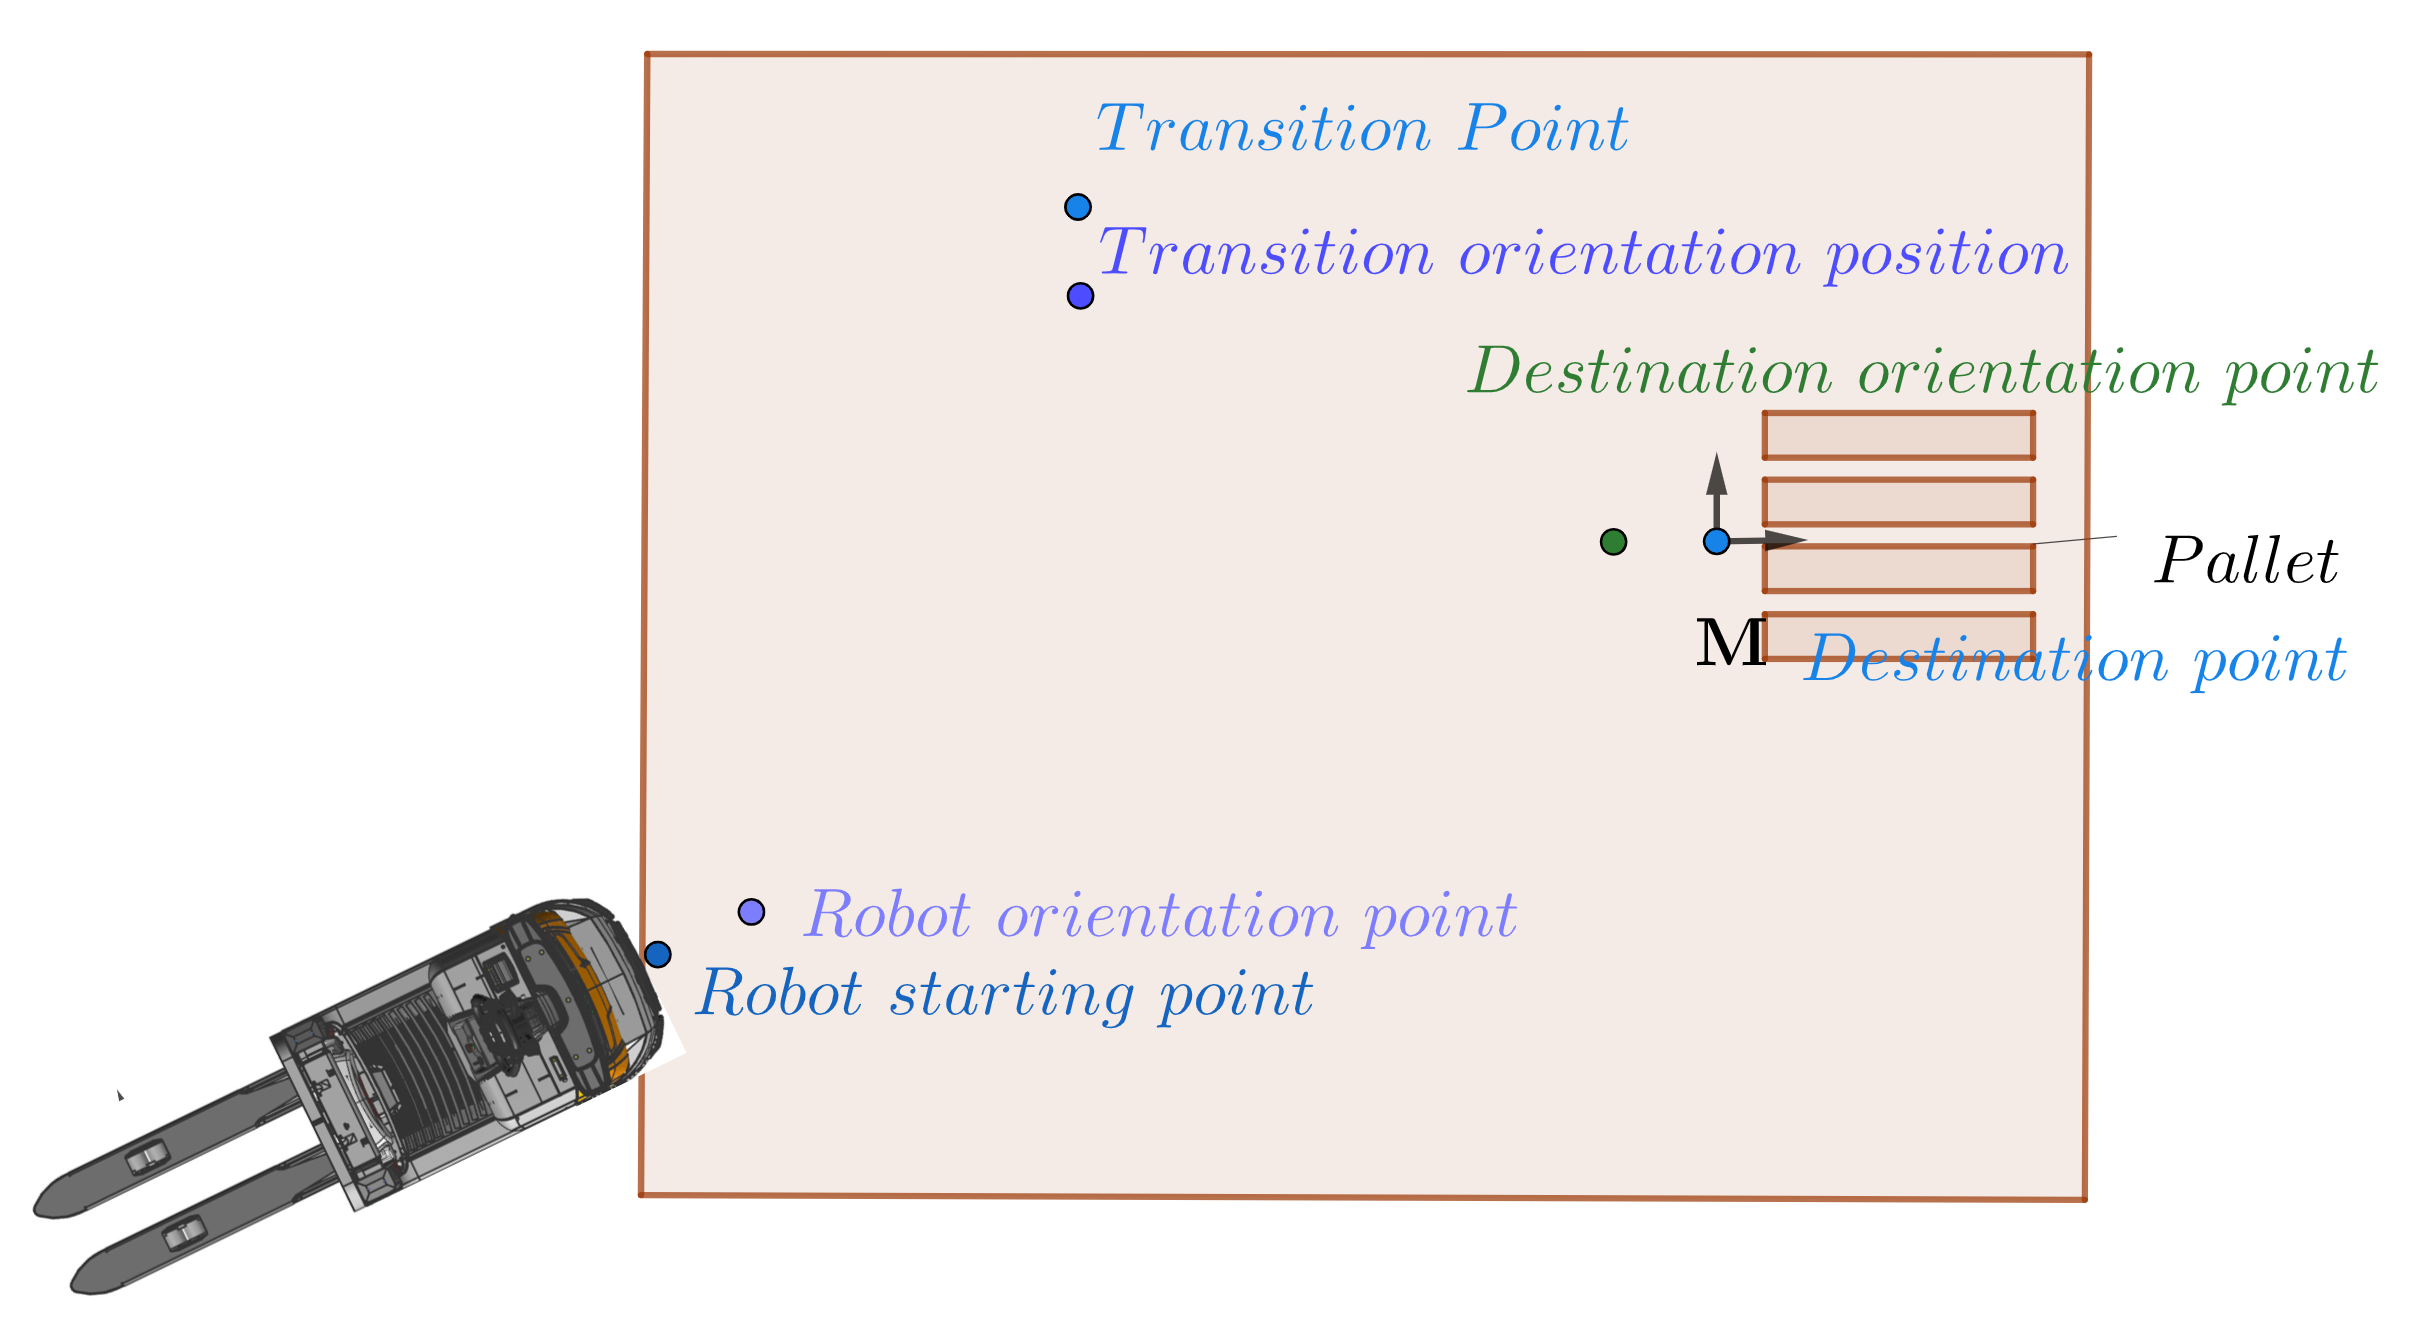
\includegraphics[width=5in]{images/Chap2/Orientation_points.png}\\
        \caption{Orientation Points}
        \label{Orientation}
        \end{center}    
\end{figure}

\begin{figure}[H]
    \begin{center}
        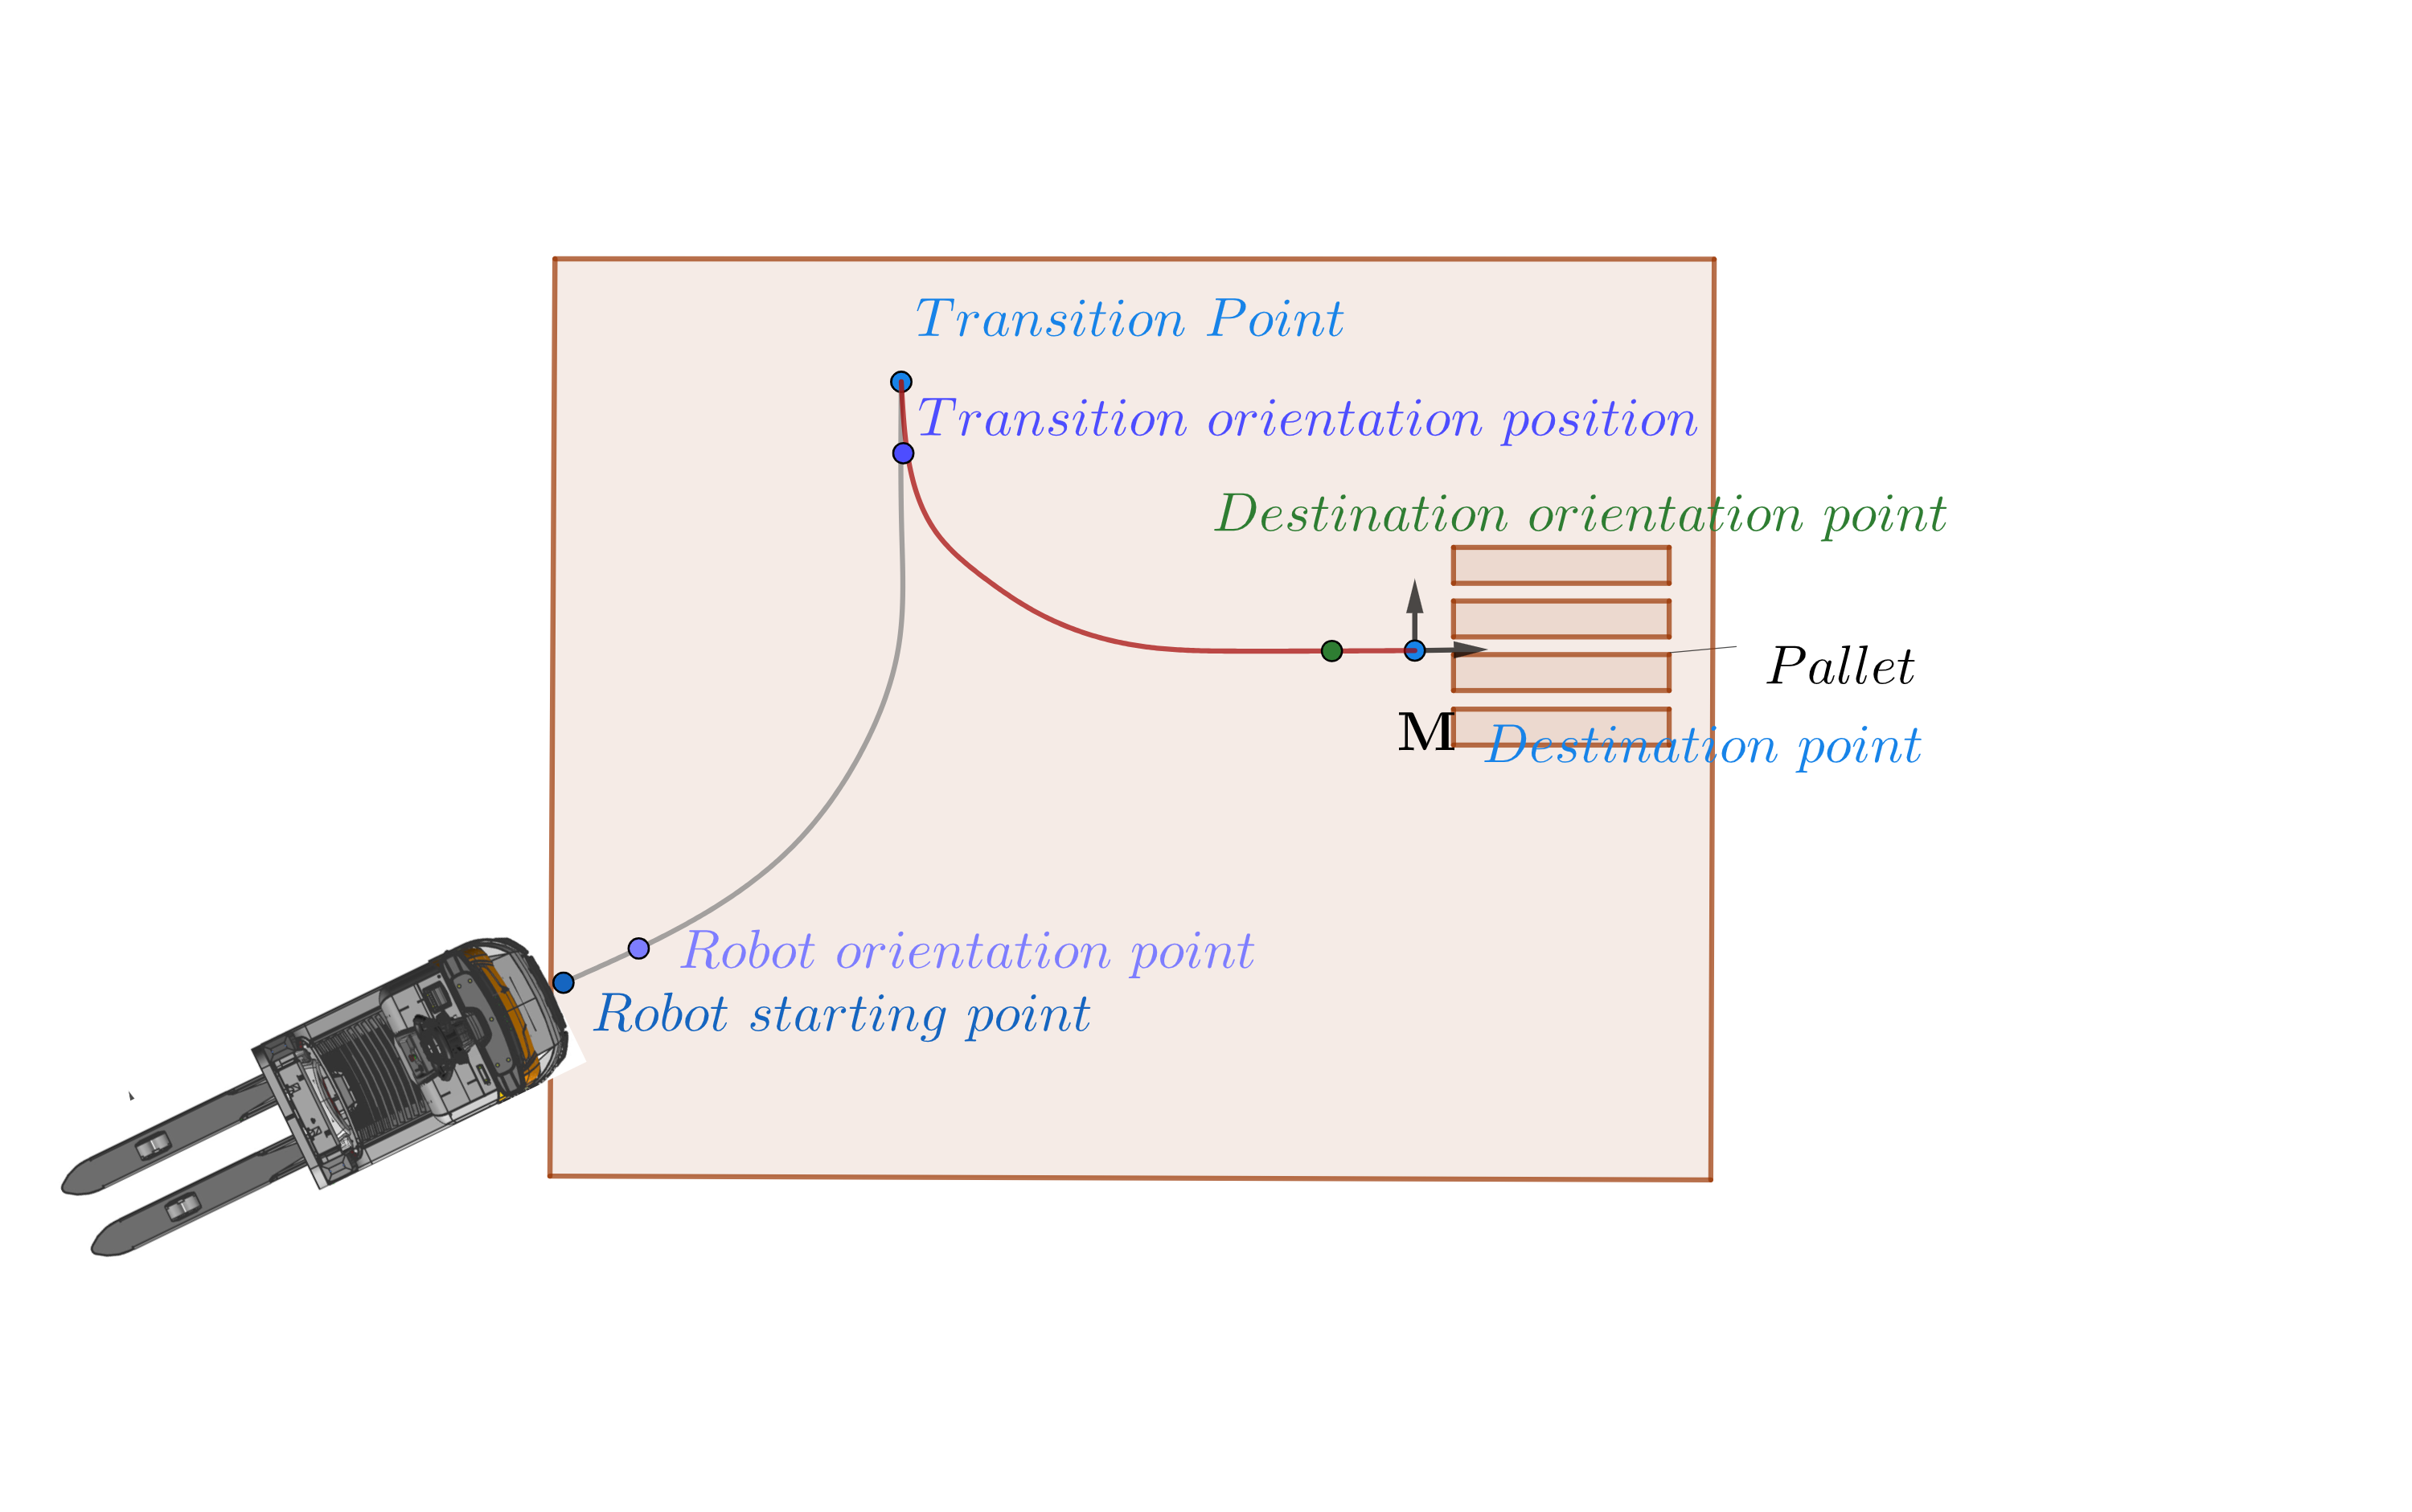
\includegraphics[width=5in]{images/Chap2/Orientation_points_with_spline.png}\\
        \caption{Interpolated Splines of Orientation points}
        \label{Spline ori}
        \end{center}    
\end{figure}

\begin{figure}[H]
    \begin{center}
        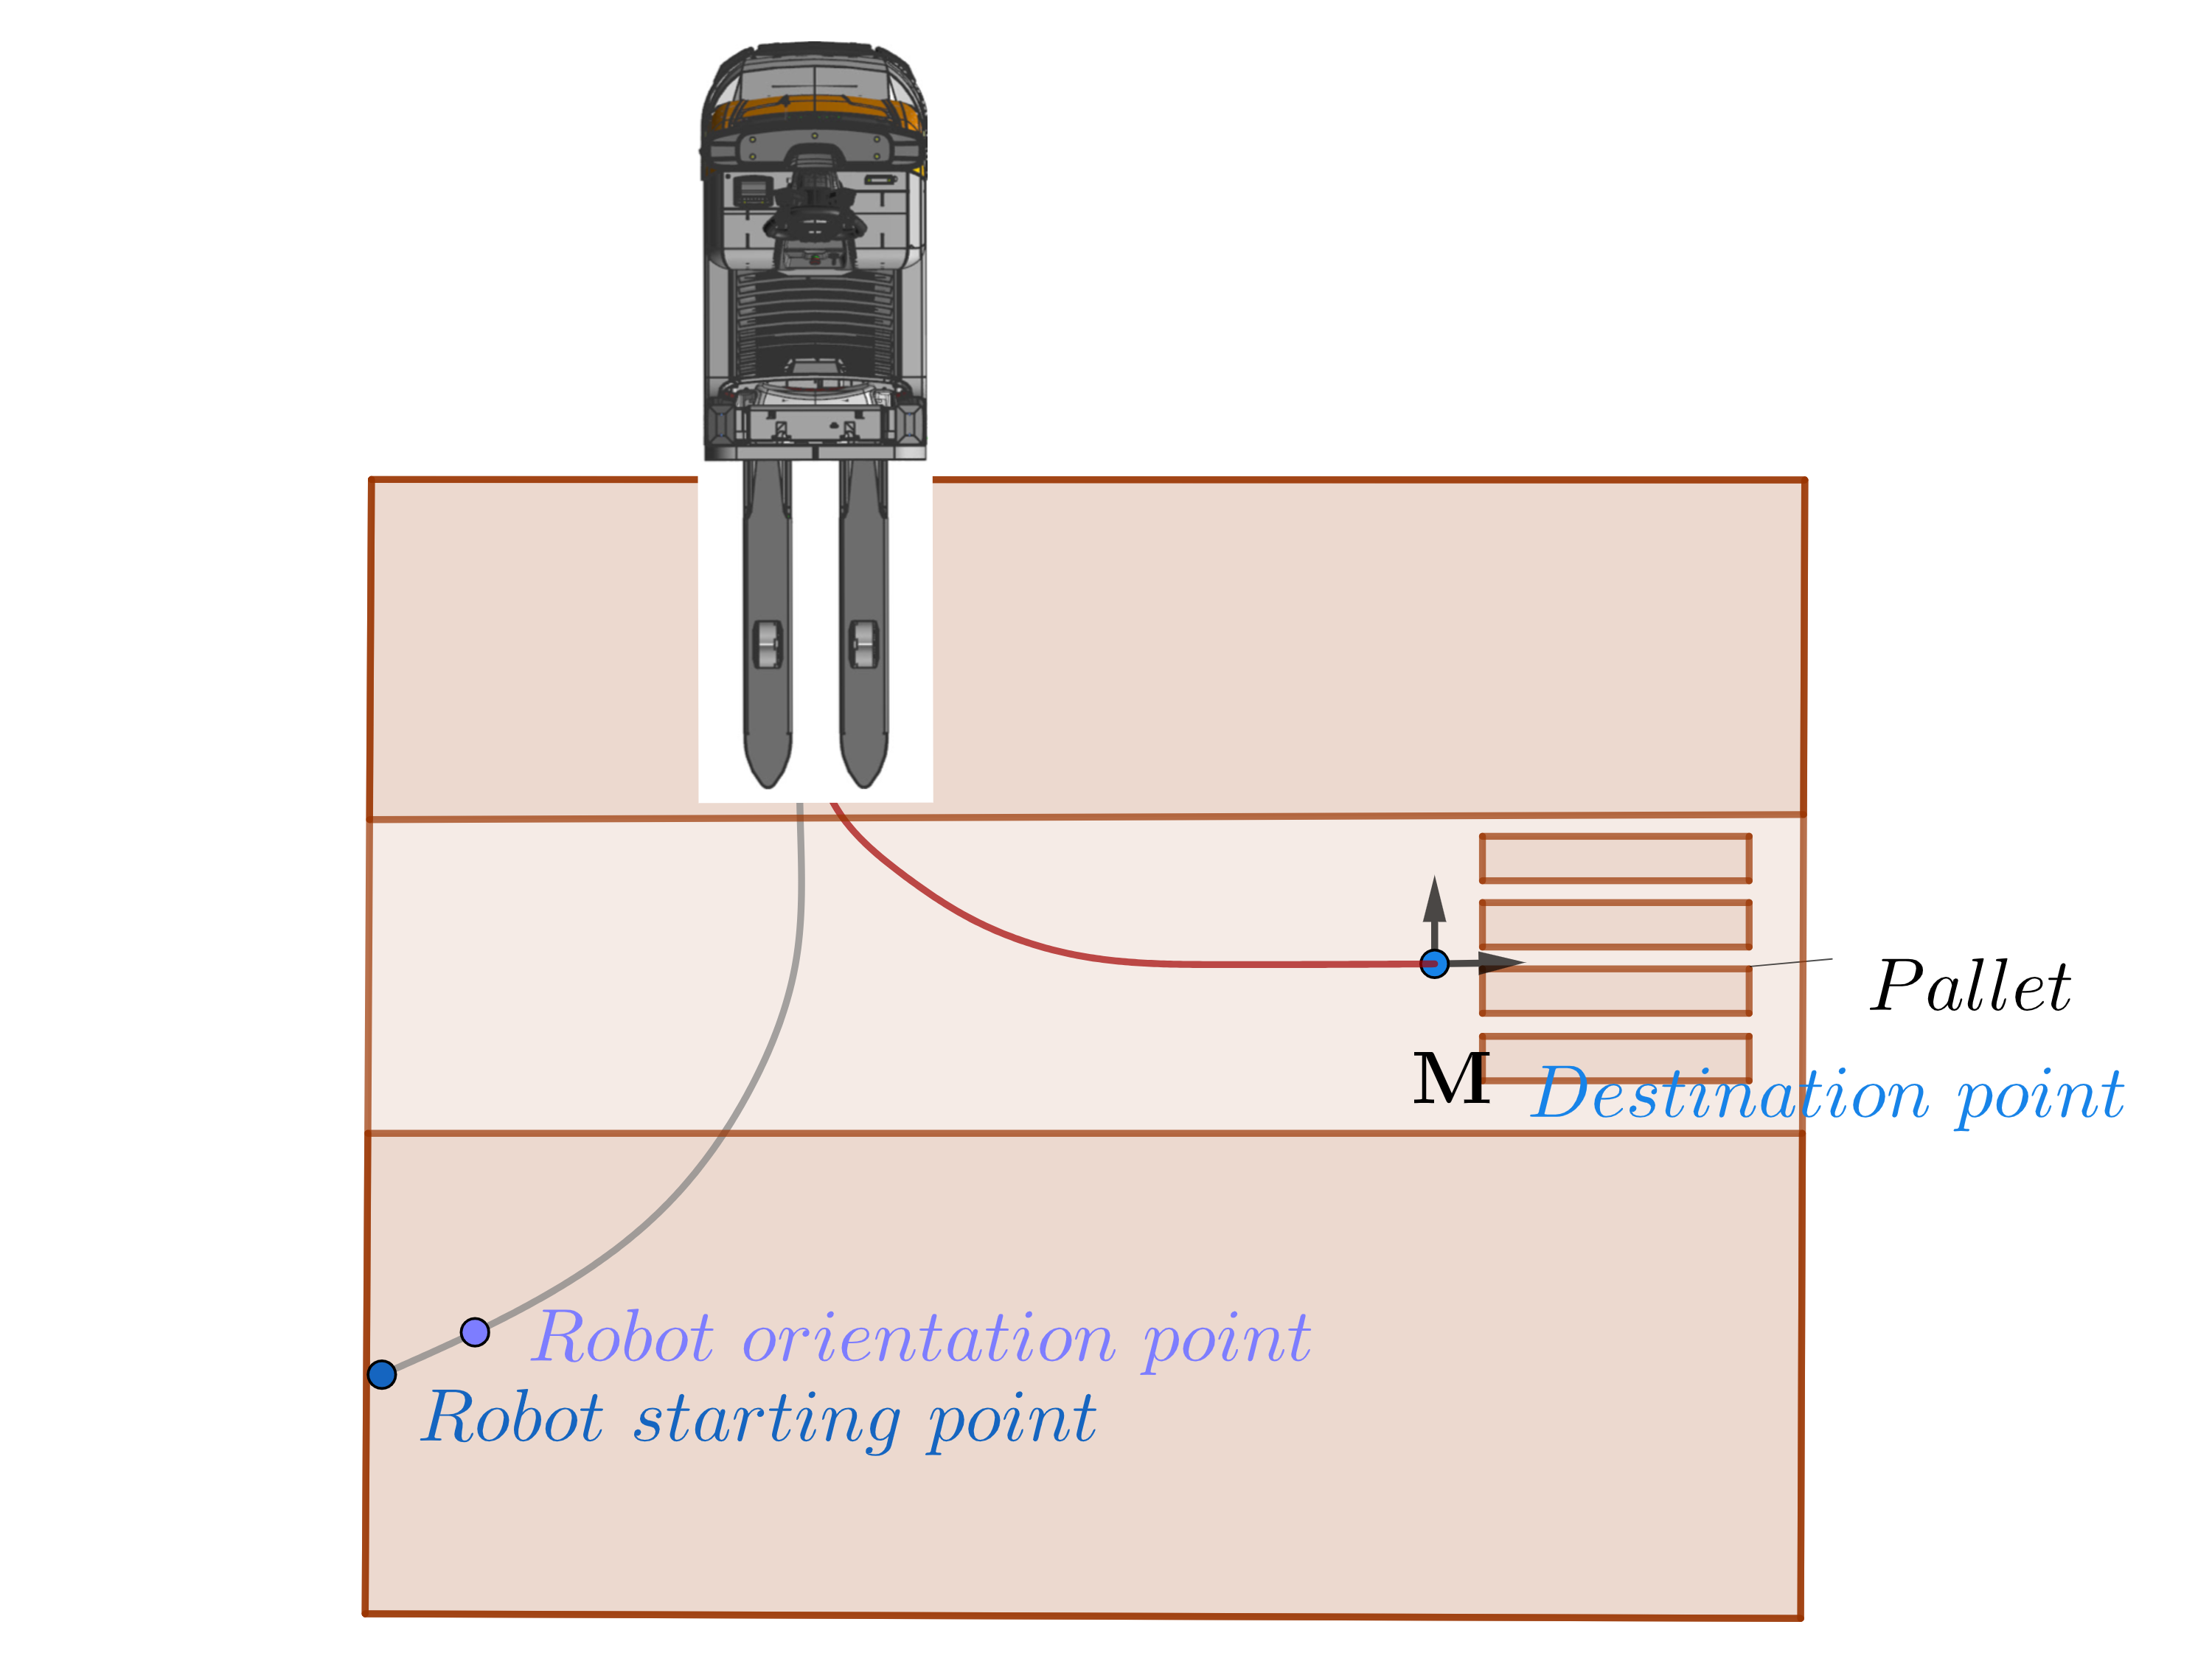
\includegraphics[width=5in]{images/Chap2/truck_transition.png}\\
        \caption{Robot at the transition position}
        \label{transition}
        \end{center}    
\end{figure}

The interpolation of the waypoints and the manipulation of splines is through The Spline Library integarted in 
the RACK framework (See RACK section%TODO add rack section
). The library provides tools to construct splines through several methods like interpolating points or blending two or more splines 
together and retrieve their features by segmeting the splines and calculating length and curvature for instance.
The result is a structure of coordinates through which passes the spline. 
The Algorithm of the approach to create a spline is explained in Pseudo code \Ref{alg:createSplines}.
The algorithm first acquires the waypoints to be interpolated. Then it creates the curve 
and measures the minimu and maximum parameter values from the knot vector which are used to evaluate 
the curve but also to retrieve relevant data about the splines like positions. It guides the exploration
of the spline. Besides, the spline length and cumulated curvature change are retrieved. 
The curvature change supervises the abrupt changes in curvature in segment curves of the whole spline.
Finally a number of positions belonging to the spline is retrieved and transfered to the path data structure,
this is where the resulting spline is transformed into a path that the robot can follow.


\begin{algorithm}[H]
    \caption{Creation of a Spline by Points Interpolation}\label{alg:createSplines}

    \SetAlgoLined
    \KwData{points}
    \KwResult{createdNewSplineFromPoints}
    
    Initialize Spline\;
    
    SetInterrogationPoints(points)\;
    CreateCurveByInterpolation()\;
    
    max\_par $\gets$ Spline.GetMaxParameterVal()\;
    min\_par $\gets$ Spline.GetMinParameterVal()\;
    length $\gets$ Spline.GetFullCordLength()\;
    curvature\_change $\gets$ Spline.GetCurvatureChange()\;
    samples $\gets$ round(length / kSegmentLength)\;
    step $\gets$ (max\_par - min\_par) / samples\;
    
    \For{f $\gets$ min\_par + step \KwTo max\_par \textbf{by} step}{
        Spline.GetPosition(f, position)\;
        PathData.Spline.Position $\gets$ position\;
    }
    
    \Return{createdNewSplineFromPoints}\;
    
    \end{algorithm}


\subsubsection{Results}
The obtained results are of smooth splines adhering to the pattern and linking the truck to the destination pallet 
while passing by a transition location. 
The simulated results of a cloned test environment show the pattern spline-based path as given by figure \Ref{Test_clone}.
The resulting path on the RACK simulation environment which is the real testing environment show as well the creation and 
plotting of the pattern path on the simulated station as given by \Ref{driving} and \Ref{Test_Simu}. 

\begin{figure}[H]
    \centering
    \begin{minipage}{0.45\textwidth}
        \centering
        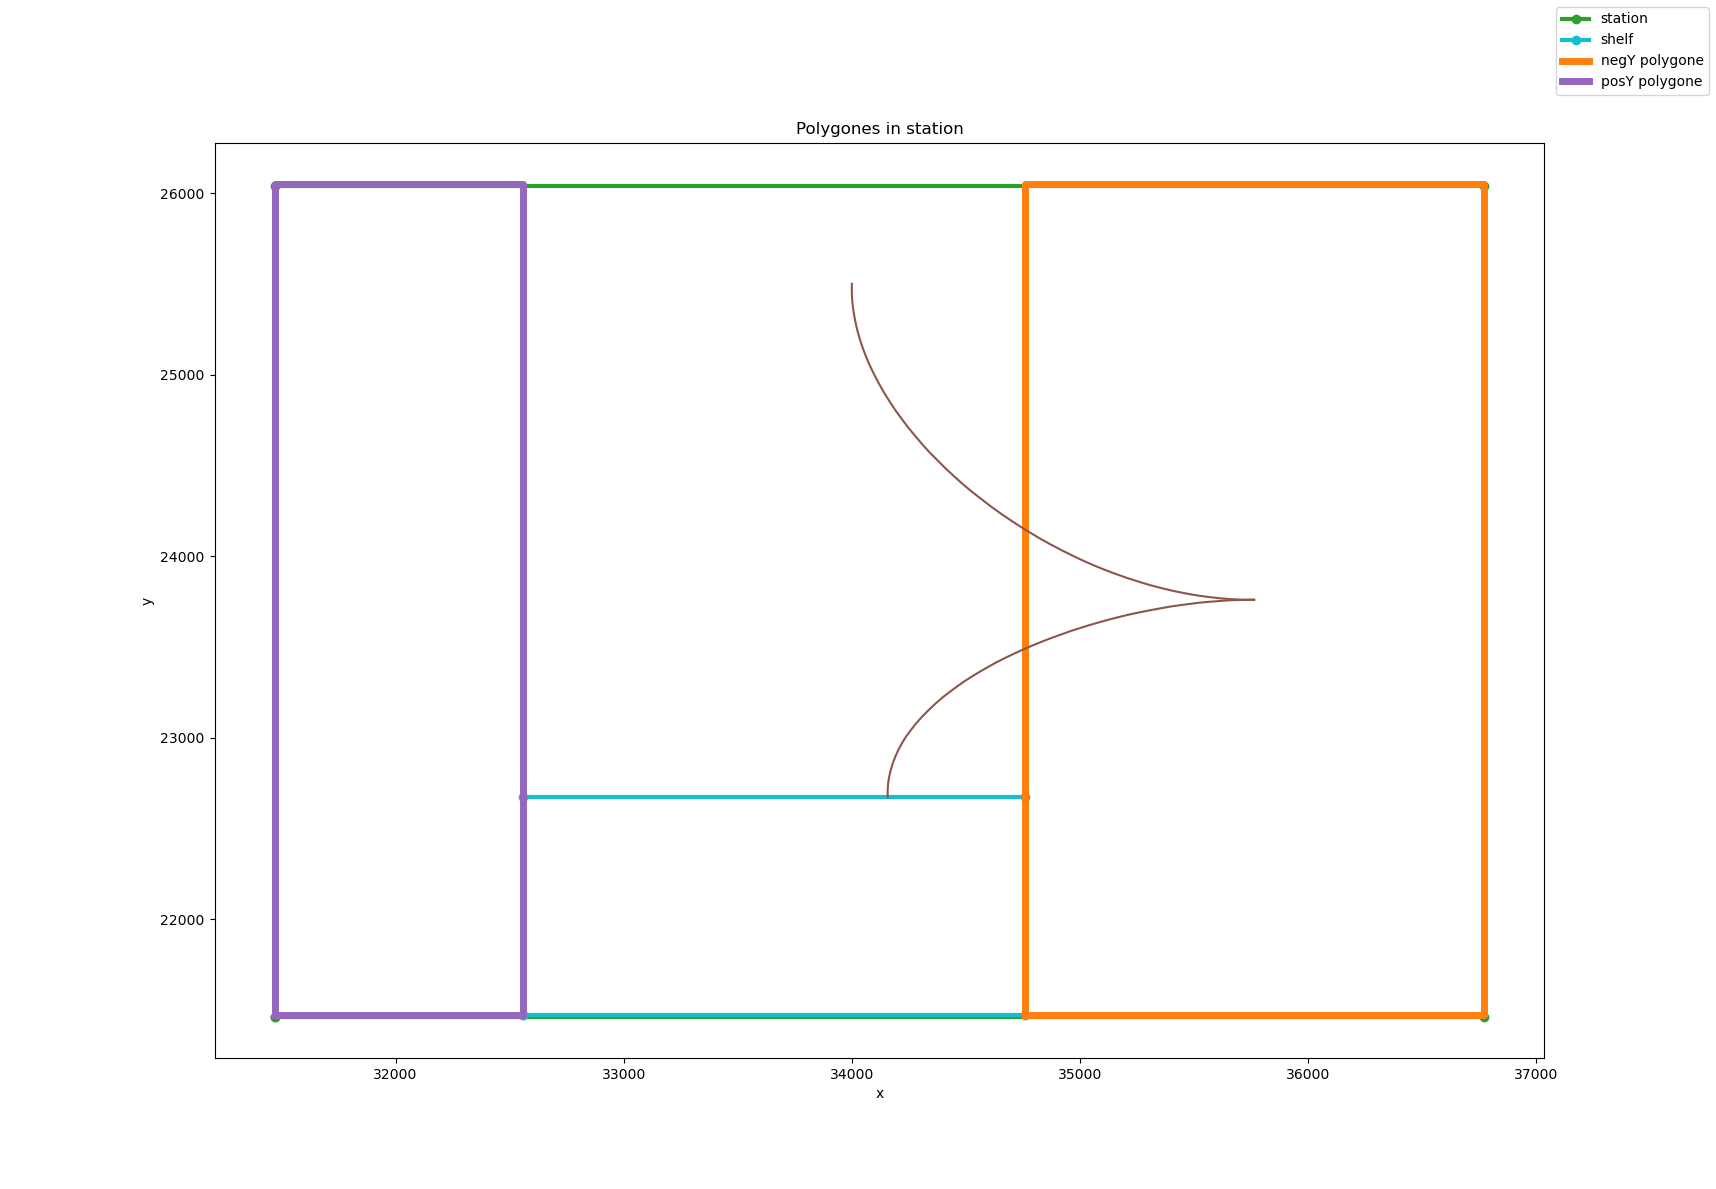
\includegraphics[width=\linewidth]{images/Chap2/spline_split.png} % Replace with your figure
    \end{minipage}
    \begin{minipage}{0.45\textwidth}
        \centering
        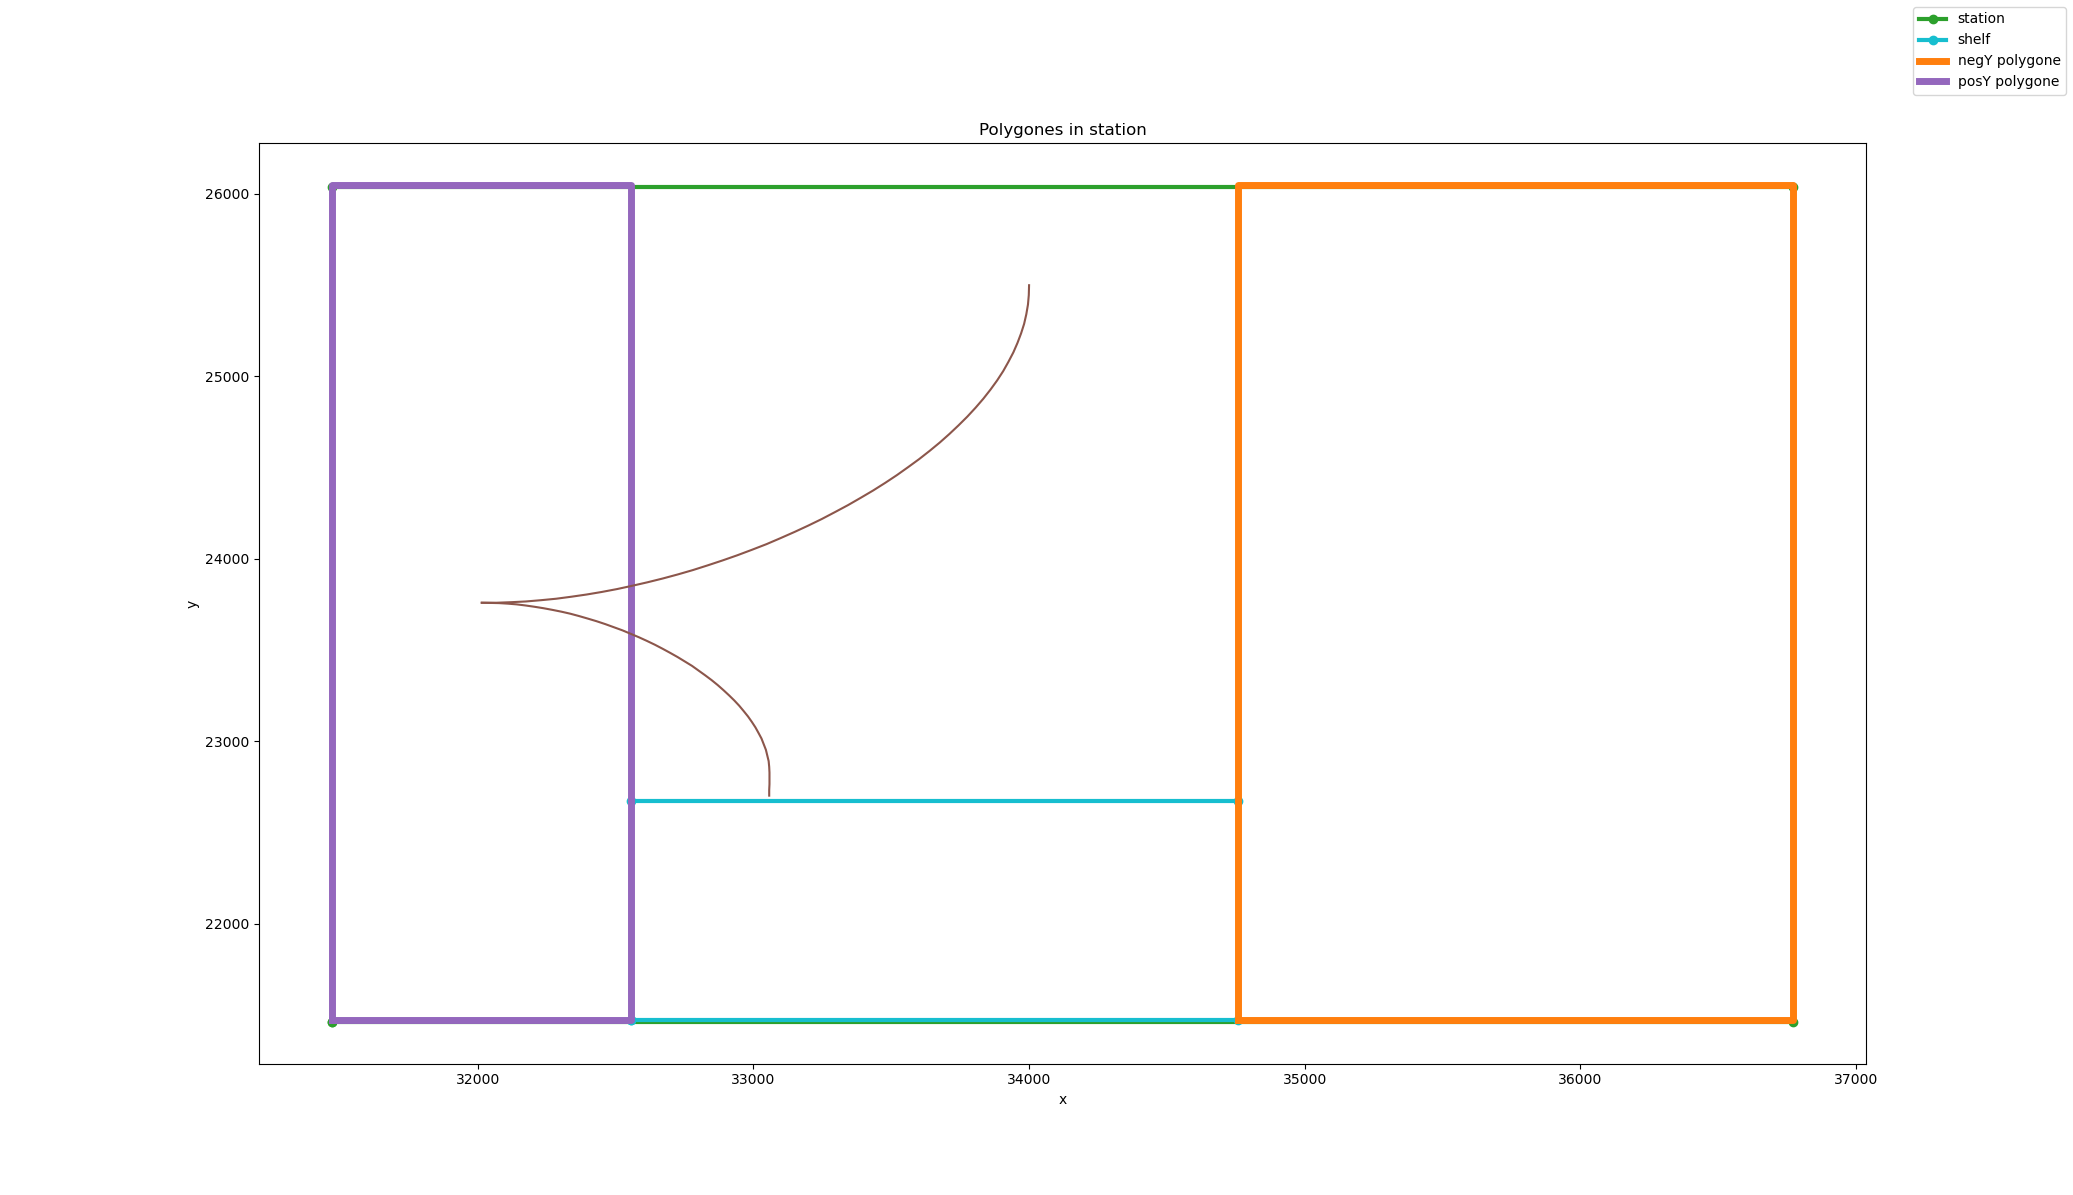
\includegraphics[width=\linewidth]{images/Chap2/spline_split_posY.png} % Replace with your figure
    \end{minipage}
    \caption{Test Results on Cloned Test Environment}
    \label{Test_clone}
\end{figure}

\begin{figure}[H]
    \begin{center}
        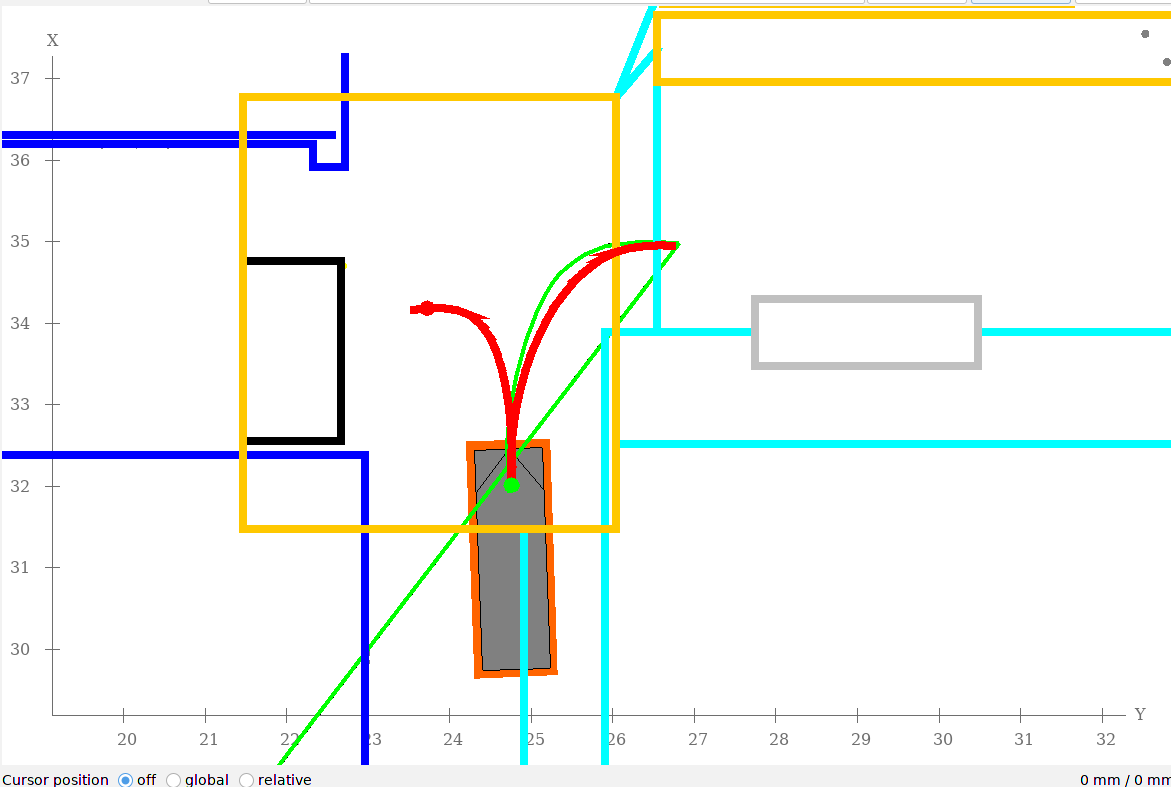
\includegraphics[width=4in]{images/Chap2/Pattern_spline_simulation_3_driving.png}\\
        \caption{Test Results on the Simulated Environment: Truck driving the Spline-based Pattern path}
        \label{driving}
        \end{center}    
\end{figure}

\begin{figure}[H]
    \centering
    \begin{minipage}{0.45\textwidth}
        \centering
        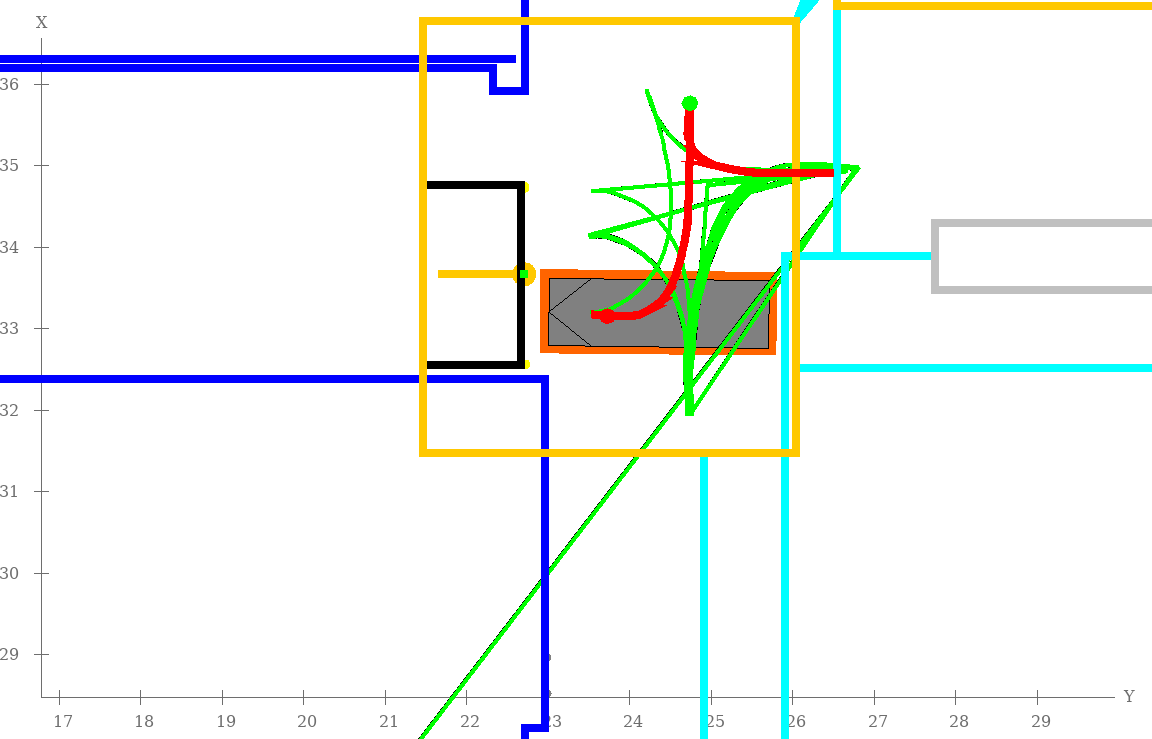
\includegraphics[width=\linewidth]{images/Chap2/Pattern_spline_simulation_1.png} % Replace with your figure
    \end{minipage}
    \begin{minipage}{0.45\textwidth}
        \centering
        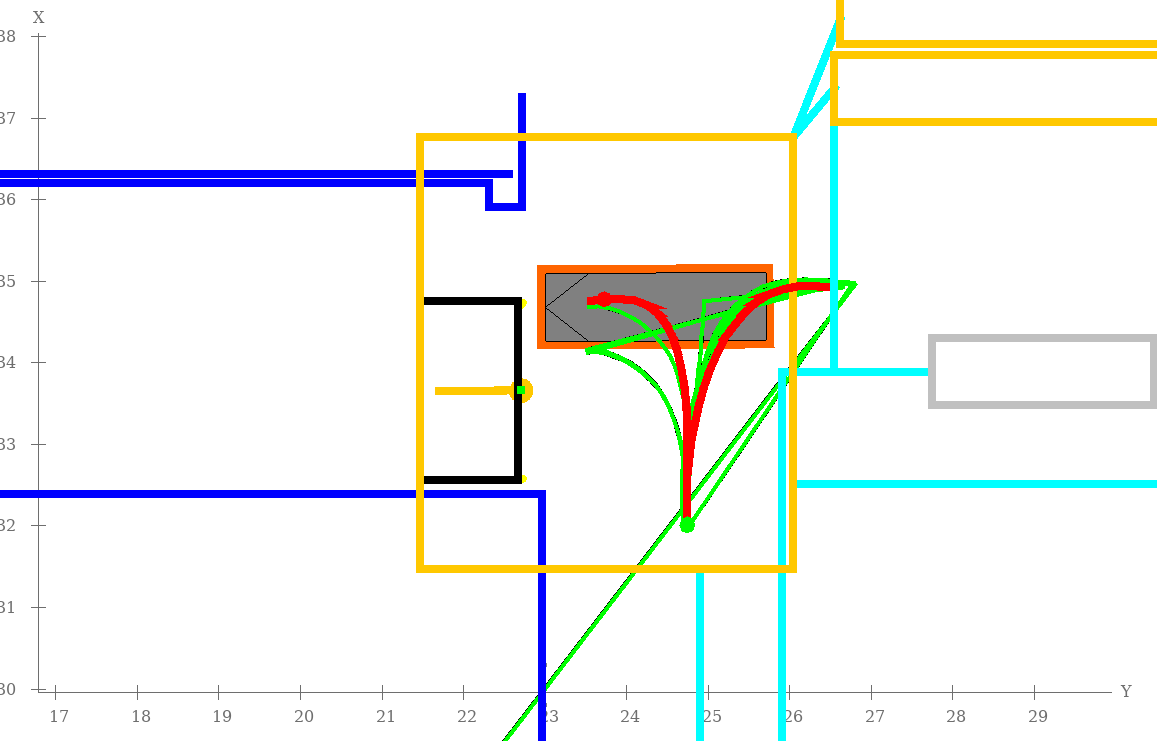
\includegraphics[width=\linewidth]{images/Chap2/Pattern_spline_simulation_2.png} % Replace with your figure
    \end{minipage}
    \caption{Test Results on the Simulated Environment: Truck at the Destination}
    \label{Test_Simu}
\end{figure}

%TODO: check if section numbers are correct: ctrl+F section
\subsection{Path Evaluation}
Once the path has been created and the relevant information has been retrieved, the foundation is set to evaluate the 
quality of the generated paths. As discussed in Section 2.3, the literature proposes several approaches to path evaluation 
that have been tested and assessed in this work. \textbf{The input for this section is a spline-based path pattern, and the 
output is a scalar value that reflects the quality of the path}.

\subsubsection{Utility}
Path evaluation allows to assess the quality of a path. From the vehicle's perspective, it enables the 
prediction of whether the path is mechanically and strategically feasible in terms of curves, sharp turns, direction 
changes, and other factors. This evaluation prevents the vehicle from following low-quality paths and paves the way 
towards optimization and selection of the best possible routes.

\subsubsection{Implementation}
By analyzing the spline,  key characteristics of the path can be determined, such as its length, curvature, and 
the time required to traverse it. The following requirements are essential for developing a robust path 
evaluation formula:
\begin{itemize}
    \item The formula used to evaluate the path must be \textbf{simple} enough to be easily integrated into an optimization process.
    During path planning, optimization algorithms are often employed to find the best possible path according to certain 
    criteria. These algorithms require objective functions that can be computed efficiently. A complex or computationally 
    expensive formula may slow down the optimization process or make it impractical for real-time applications. 
    Therefore, the path evaluation formula should be simple, allowing for quick calculations that can be repeatedly 
    applied within an optimization loop. This simplicity also facilitates its integration with existing optimization 
    frameworks.
    \item The formula should include a \textbf{normalization} step to ensure that different paths can be compared on a common scale.
    Paths can vary significantly in terms of length, curvature, and other characteristics. To make meaningful 
    comparisons between paths, it’s essential to normalize these metrics. Normalization involves scaling the values of 
    each metric (e.g., path length, curvature change) relative to a reference value, such as the characteristics of 
    a potential ideal path. By normalizing the path metrics, it is ensured that the evaluation formula is 
    dimensionless and that the different aspects of the path (e.g., length versus curvature) are balanced 
    appropriately. This step is crucial when combining multiple metrics into a single evaluation score, as it 
    prevents any one metric from disproportionately influencing the final result.
    \item The evaluation should \textbf{prioritize paths that minimize length and curvature}.  In most path planning scenarios, 
    especially for vehicles or robots, the goal is to find the most efficient path from point A to point B. 
    Efficiency can be measured in terms of:
    \begin{itemize}
        \item Path Length: Shorter paths are generally preferred because they reduce the distance the vehicle or robot 
        needs to travel, therefore saving energy and time.
        \item Curvature: Paths with less curvature are preferred because sharp turns can be difficult for vehicles 
        to navigate, especially at higher speeds. Minimizing curvature reduces the risk of instability of the vehicle.
    \end{itemize}
    
\end{itemize}

The combination of these requirements leads to a path evaluation formula that is both practical and effective. 

To implement this path evaluation effectively, it was essential to accurately measure the path's length and curvature 
change, as these are critical components of the evaluation formula. 

The path length was calculated by summing the distances between consecutive points along the spline, ensuring that 
even small variations in the path's trajectory were captured as given by equation \Ref{length_formula}.
\begin{equation}
    L = \sum_{i=\min \ \text{par}}^{\max \ \text{par}} s(i)
    \label{length_formula}
\end{equation}
where \( s(i) \) denotes the length of the \(i\)-th curve segment of the spline measured between two points of the 
spline using Euclidean distance.

The curvature change of a spline path is quantified by evaluating how the curvature of the path varies along its Length.
The curvature change (\( cc \)) calculated by:

\begin{equation}
cc = \int \frac{d(k)}{d(s)} \, ds
\end{equation}

represents the total variation in curvature along the path, where \( \frac{d(k)}{d(s)} \) measures how curvature itself 
changes as a function of arc length, and integrating this derivative over the path provides a comprehensive metric of 
curvature variation.

As this equation involves an integral, it has to be approximated in order to compute it in a programming environment.
The approximation is conducted through a discretization of the path into a series of small segments. For each segment, 
the curvature change and segment length are approximated. Let \( \Delta s(i) \) denote the length of the \(i\)-th segment 
and \( \Delta k(i) \) the change in curvature over this segment.
Then, the trapezoidal rule is used to approximate the integral. 
This is achieved by summing up the ratio of curvature change to segment length over all segments as given by 
equation \Ref{curvature_change}:
\begin{equation}
cc = \sum_{i = \min \ \text{par} + \text{step}}^{\max \ \text{par}} \frac{\Delta k(i)}{\Delta s(i)}
\label{curvature_change}
\end{equation}

Mathematically, if \(k(i)\) is the curvature at the \(i\)-th segment, then \( \Delta k(i) \) can be expressed as:
\begin{equation}
    \Delta k(i) = \left| k(i) - k(i-1) \right|
\end{equation}
where \(k(i-1)\) is the curvature of the previous segment. The absolute value is used to prevent cancellation of terms:
curvature can be negative or positive according to the convexity or concavity of the curve. When summed together,
a neutralization could happen resulting in an insignificant value. This could be solved by introducing the squarred 
difference between \(k(i)\) and \(k(i-1)\). However, it will minimize the result to a negligible value for the 
overall analysis as the curvature values are around the magnitude of \(10^{-2}\) or less.

The summation provides a cumulative measure of curvature changes relative to the segment lengths along the entire path, 
offering insight into the overall curvature dynamics of the spline. The formula for \(cc\) evaluates the total effect 
of curvature changes normalized by segment lengths over 
the path. This metric is useful for understanding how the path’s curvature varies and helps in optimizing paths 
to ensure smooth and efficient navigation.

To develop a cost function that integrates both path length and curvature, we explore two distinct approaches: 
Exponential Weighted Path Evaluation and Normalized Weighted Path Evaluation. These approaches use weights to 
prioritize the significance of each component in the evaluation process. 

\subsubsubsection{First approach: Exponential Weighted Path Evaluation}
The Exponential Path Evaluation is based on A. Elshamli, et al. method \cite{R17}. As explained in section 2.3,
they consider path length, smoothness and clearance combined in a weighted cost function.
Their approach of measuring path length and smoothness is considered here with some changes to fit it into the use case.

Path length term is measured in \cite{R17} as follows:
\begin{equation}
d = \sum_{i=1}^{n-1} d(s_i)
\end{equation}

Whereas, Path smoothness is measured as follows:

\begin{equation}
d = \sum_{i=2}^{n-1} \exp(a(\theta_i - \alpha))
\end{equation}

where \( \theta_i \) represent the steering angle at the \(i\)-th segment, and \( \alpha \) denote the desired 
steering angle.

Besides path clearance, those values are weighted and summed.
This summation is not normalized given that it adds the distance term which has a unit to the smoothness and 
clearance terms that are exponential functions results. 
In this approach of the work, the exponential function is used for normalization of distance and curvature change 
terms. The length term is given by:
\begin{equation}
    \text{Length Term} = e^{\beta \cdot \left(\text{current}_L - \text{ref}_L\right)}
    \end{equation}
    
    \noindent
    The curvature change term is given by:
    \noindent
    
    \begin{equation}
    \text{Curvature Change Term} = e^{\alpha \cdot \left(\text{current}_{cc} - \text{ref}_{cc}\right)}
    \end{equation}
    
    \noindent
    where: 
    \newline
    - \textit{current} refers to the path being evaluated and \textit{ref} refers to the reference path.
    \newline
    - \(\alpha\) and \(\beta\) are factors that rationalize the exponential terms because the length is in the range 
    of thousands of millimeters while the curvature is around the magnitude of \(10^{-2}\) or less.
    Without these factors, the two terms would differ significantly, leading to incorrect analysis of the impact of each term.
    
\noindent The cost function of the weighted terms is given by equation \Ref{exp_function}:

\begin{equation}
Z^{\ast }=\arg \min \left(\omega_{c} \cdot e^{\alpha \cdot \left( \text{current}_{cc} - \text{ref}_{cc} \right)} + \omega_{L} 
\cdot e^{\beta \cdot \left( \text{current}_L - \text{ref}_L \right)} \right)
\label{exp_function}
\end{equation}
\noindent
with constraints: \[K(i)\ <\ K_{\max}\]
\noindent

and \[\text{RobotFootprint}(\mathbf{p}_i) = 0 \quad \text{for all } i\]


where \begin{itemize}
    \item \(\omega_c\) and \(\omega_L\) are the weights assigned to the curvature change term and the length term, 
    respectively. These weights determine the relative importance of curvature change and path length in the overall 
    evaluation. 
    \item \(\ K_{\max}\) the maximum tolerated curvature
    \item \( \mathbf{p}_i \) represent the \( i \)-th scan point in space. 

    \item \( \text{RobotFootprint}(\mathbf{p}_i) \) be a boolean function that returns 1 if the point \( \mathbf{p}_i \) 
    lies within the robot's footprint (polygon) and 0 otherwise.
    
\end{itemize}


\subsubsubsection{Second approach: Normalized Weighted Path Evaluation}

The Normalized Weighted Path Evaluation is based on the division of the path's Length
and Curvature Change measured respectively using the equations \Ref{Length_formula} and 
\Ref{curvature_change} respectively by the reference path's Length and Curvature Change. 
The length term is given by:
\begin{equation}
    \text{Length Term} = \frac{\sum_{i=\min \text{ par}}^{\max \text{ par}} s(i)_j}{\sum_{i=\min \text{ par}}^{\max \text{ par}} s(i)_{\text{ref}}}
\end{equation}

\noindent
The curvature change term is given by:

\begin{equation}
    \text{Curvature Change Term} = \frac{\sum_{i=j \min \text{ par}}^{j \max \text{ par}} \frac{\Delta k(i)_j}{\Delta s(i)_j}}{\sum_{i=\text{ref} \min \text{ par}}^{\text{ref} \max \text{ par}} \frac{\Delta k(i)_{\text{ref}}}{\Delta s(i)_{\text{ref}}}}
\end{equation}

where \( j \) denotes the current path being evaluated.

\noindent The cost function of the weighted terms is given by equation \Ref{Norm_function}:
\begin{equation}
    Z^{\ast} = \arg \min \left( \omega_C \cdot \frac{\sum_{i=\text{j min par}}^{\text{j max par}} \frac{\Delta k(i)_j}
    {\Delta s(i)_j}}{\sum_{i=\text{ref min par}}^{\text{ref max par}} \frac{\Delta k(i)_{\text{ref}}}
    {\Delta s(i)_{\text{ref}}} } + \omega_L \cdot \frac{\sum_{i=\text{min par}}^{\text{max par}} s(i)_j}
    {\sum_{i=\text{min par}}^{\text{max par}} s(i)_{\text{ref}}} \right)
\label{Norm_function}
\end{equation}

\noindent
with constraints: \[K(i)\ <\ K_{\max}\]
\noindent

and \[\text{RobotFootprint}(\mathbf{p}_i) = 0 \quad \text{for all } i\]


where \begin{itemize}
    \item \(\omega_c\) and \(\omega_L\) are the weights assigned to the curvature change term and the length term, 
    respectively. These weights determine the relative importance of curvature change and path length in the overall 
    evaluation. 
    \item \(\ K_{\max}\) the maximum tolerated curvature
    \item \( \mathbf{p}_i \) represent the \( i \)-th scan point in space. 

    \item \( \text{RobotFootprint}(\mathbf{p}_i) \) be a boolean function that returns 1 if the point \( \mathbf{p}_i \) 
    lies within the robot's footprint (polygon) and 0 otherwise.
    
\end{itemize}

The algorithm that measures the path quality is detailed through Pseudo Code \Ref{EvaluationAlgorithm}.

\subsubsection{Results}
Both evaluation approaches were tested in the cloned simulation environment. 
Tests were ran on 10 different spline paths  that were generated with transition points scattered in the station \Ref{Mult_splines}.
Different locations were used to stress the metric outcomes. 
The Exponential Weighted Path Evaluation was tested with \(\alpha\) = \(2\), \(\beta\) = \(0.0007\), 
\(\omega_c\)= \(0.7\) and \(\omega_L\)=\(0.3\).
The results are shown in figure \Ref{Test_Eval_Exp}

\begin{figure}[H]
    \begin{center}
        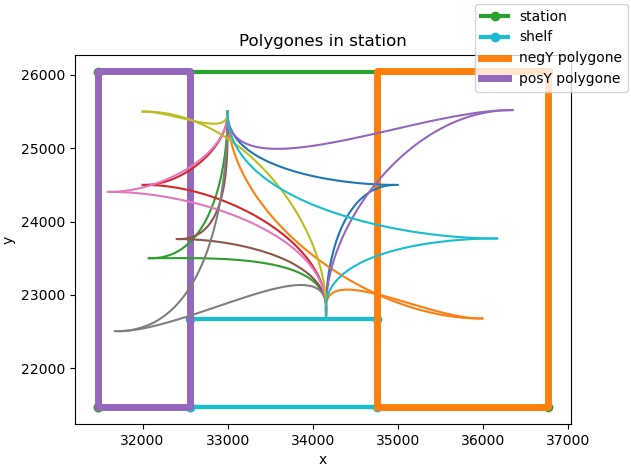
\includegraphics[width=4in]{images/Chap2/Mult_Splines.png} % Replace with your figure
        \caption{Test Results on the Simulated Environment: Multiple Splines Visualization}
        \label{Mult_splines}
        \end{center}    
\end{figure}

\begin{figure}[H]
    \begin{center}
        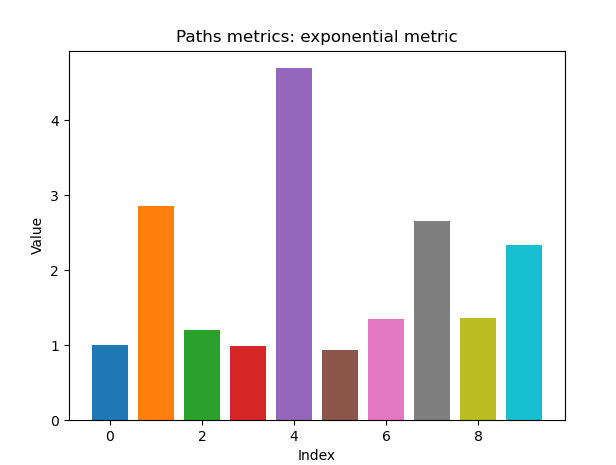
\includegraphics[width=4in]{images/Chap2/Exp_Results.png} % Replace with your figure
        \caption{Test Results on the Simulated Environment: Evaluation results of the Exponential Approach}
        \label{Test_Eval_Exp}
        \end{center}    
\end{figure}

The Normalized Weighted Path Evaluation was ran for two tests on the same splines set with 
\(\omega_c\)= \(0.7\) and \(\omega_L\)=\(0.3\) as well as 
\(\omega_c\)= \(0.5\) and \(\omega_L\)=\(0.5\). 
The results are shown in figures \Ref{Test_Eval_Norm1} and \Ref{Test_Eval_Norm2}

\begin{figure}[H]
    \begin{center}
        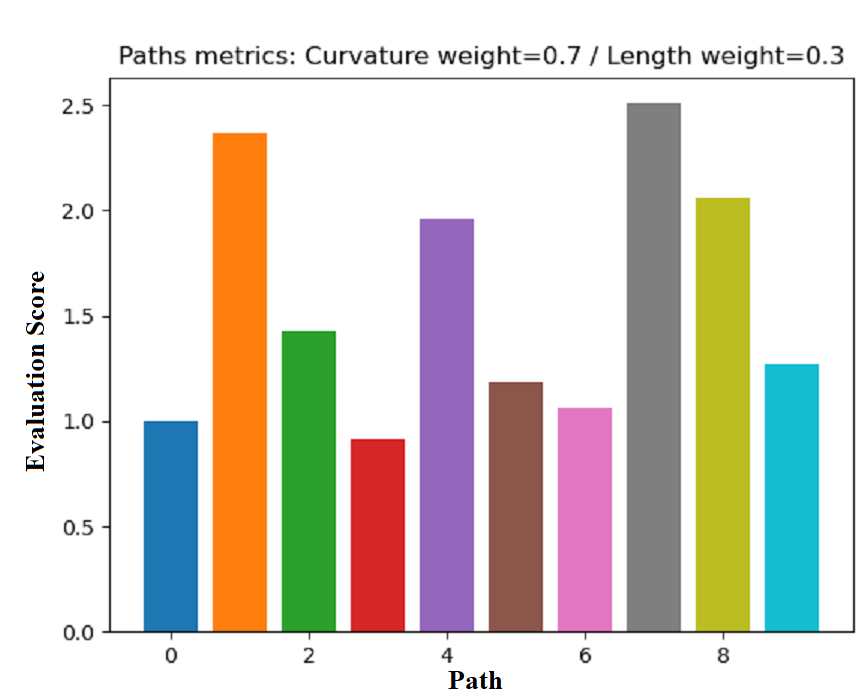
\includegraphics[width=4in]{images/Chap2/w_0.7.png} % Replace with your figure
        \caption{Test Results on the Simulated Environment: Evaluation results of the Normalized Approach
        with weighing out the curvature}
        \label{Test_Eval_Norm1}
        \end{center}    
\end{figure}
\begin{figure}[H]
    \begin{center}
        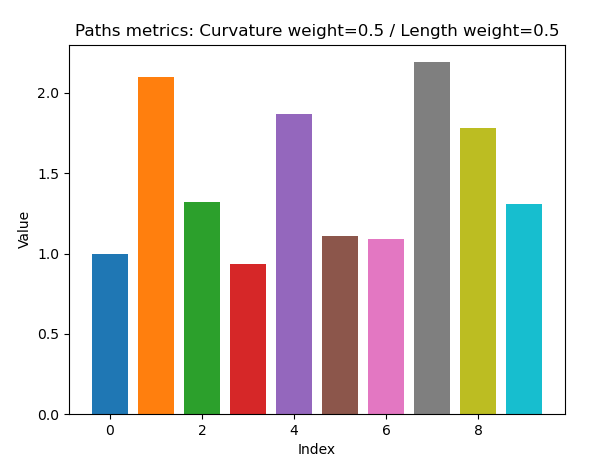
\includegraphics[width=4in]{images/Chap2/w_0.5.png} % Replace with your figure
        \caption{Test Results on the Simulated Environment: Evaluation results of the Normalized Approach
        with equal weights}
        \label{Test_Eval_Norm2}
        \end{center}    
\end{figure}



\begin{algorithm}[H]
    \caption{Path Evaluation Algorithm}\label{EvaluationAlgorithm}

    \SetAlgoLined
    \KwData{Spline Path, set of scan points $P$}
    \KwResult{Evaluation result}
    
    Initialize Metric\;
    
    \If{local\_max\_curvature > maximum\_curvature\_}{
        metric.curvature\_change\_ $\gets$ curvature\_KnockOut\_factor $\cdot$ local\_curv\_change\;
    }
    \Else{
        metric.curvature\_change\_ $\gets$ local\_curv\_change\;
    }
    
    metric.length\_ $\gets$ metric.calculate\_length\_metric(gen)\;
    
    \For{each point $p_i$ in $P$}{
        test $\gets$ RobotFootprint($p_i$)\;
        
        \If{test == 0}{
            result $\gets$ obstacle\_KnockOut\;
        }
        \Else{
            result $\gets$ EvaluationFunction(curvature, length)\;
        }
    }
    
    \Return{result}\;
\end{algorithm}

